\chapter{注意力和动作的视觉处理} \label{chap:chap25}

人脑具有惊人的能力,可以将注意力引导到视觉世界中的物体上,比如一个婴儿伸手去拿物体,一个网球运动员击球,一个艺术家看模特。
这种能力需要视觉系统解决三个问题:
对视觉世界进行空间精确分析,从视觉世界的混乱刺激中选择感兴趣的物体,并将物体的位置和细节信息传递给运动系统。



\section{大脑补偿眼球运动以创建视觉世界的稳定表示}

尽管视觉系统可以生动地再现我们的视觉世界,如前几章所述,但视觉图像不像瞬时摄影记录,而是根据眼睛的几个离散神经通路传递的信息动态构建的。
例如,当我们看一幅画时,我们会通过一系列快速的眼球运动(扫视)来探索它,这些运动会将中央凹重新定向到视野中感兴趣的不同物体。
在从视网膜中的光刺激产生可解释的视觉图像的过程中,大脑必须考虑到这些眼球运动。


当每个扫视将一个新物体带到中央凹时,整个视觉世界的图像都会在中央凹上发生变化。
这些变化每秒发生几次,以至于几分钟后运动记录变得混乱(图~\ref{fig:25_1})。
通过这种不断的移动,视觉图像应该类似于业余视频,其中图像会四处晃动,因为摄像师不熟练地保持相机稳定。
然而,事实上我们的视觉是如此稳定,以至于我们通常不会意识到\textit{扫视}的视觉效果。
之所以如此,是因为大脑在每次扫视后都会对落在视网膜上的图像进行持续调整。


\begin{figure}[htbp]
	\centering
	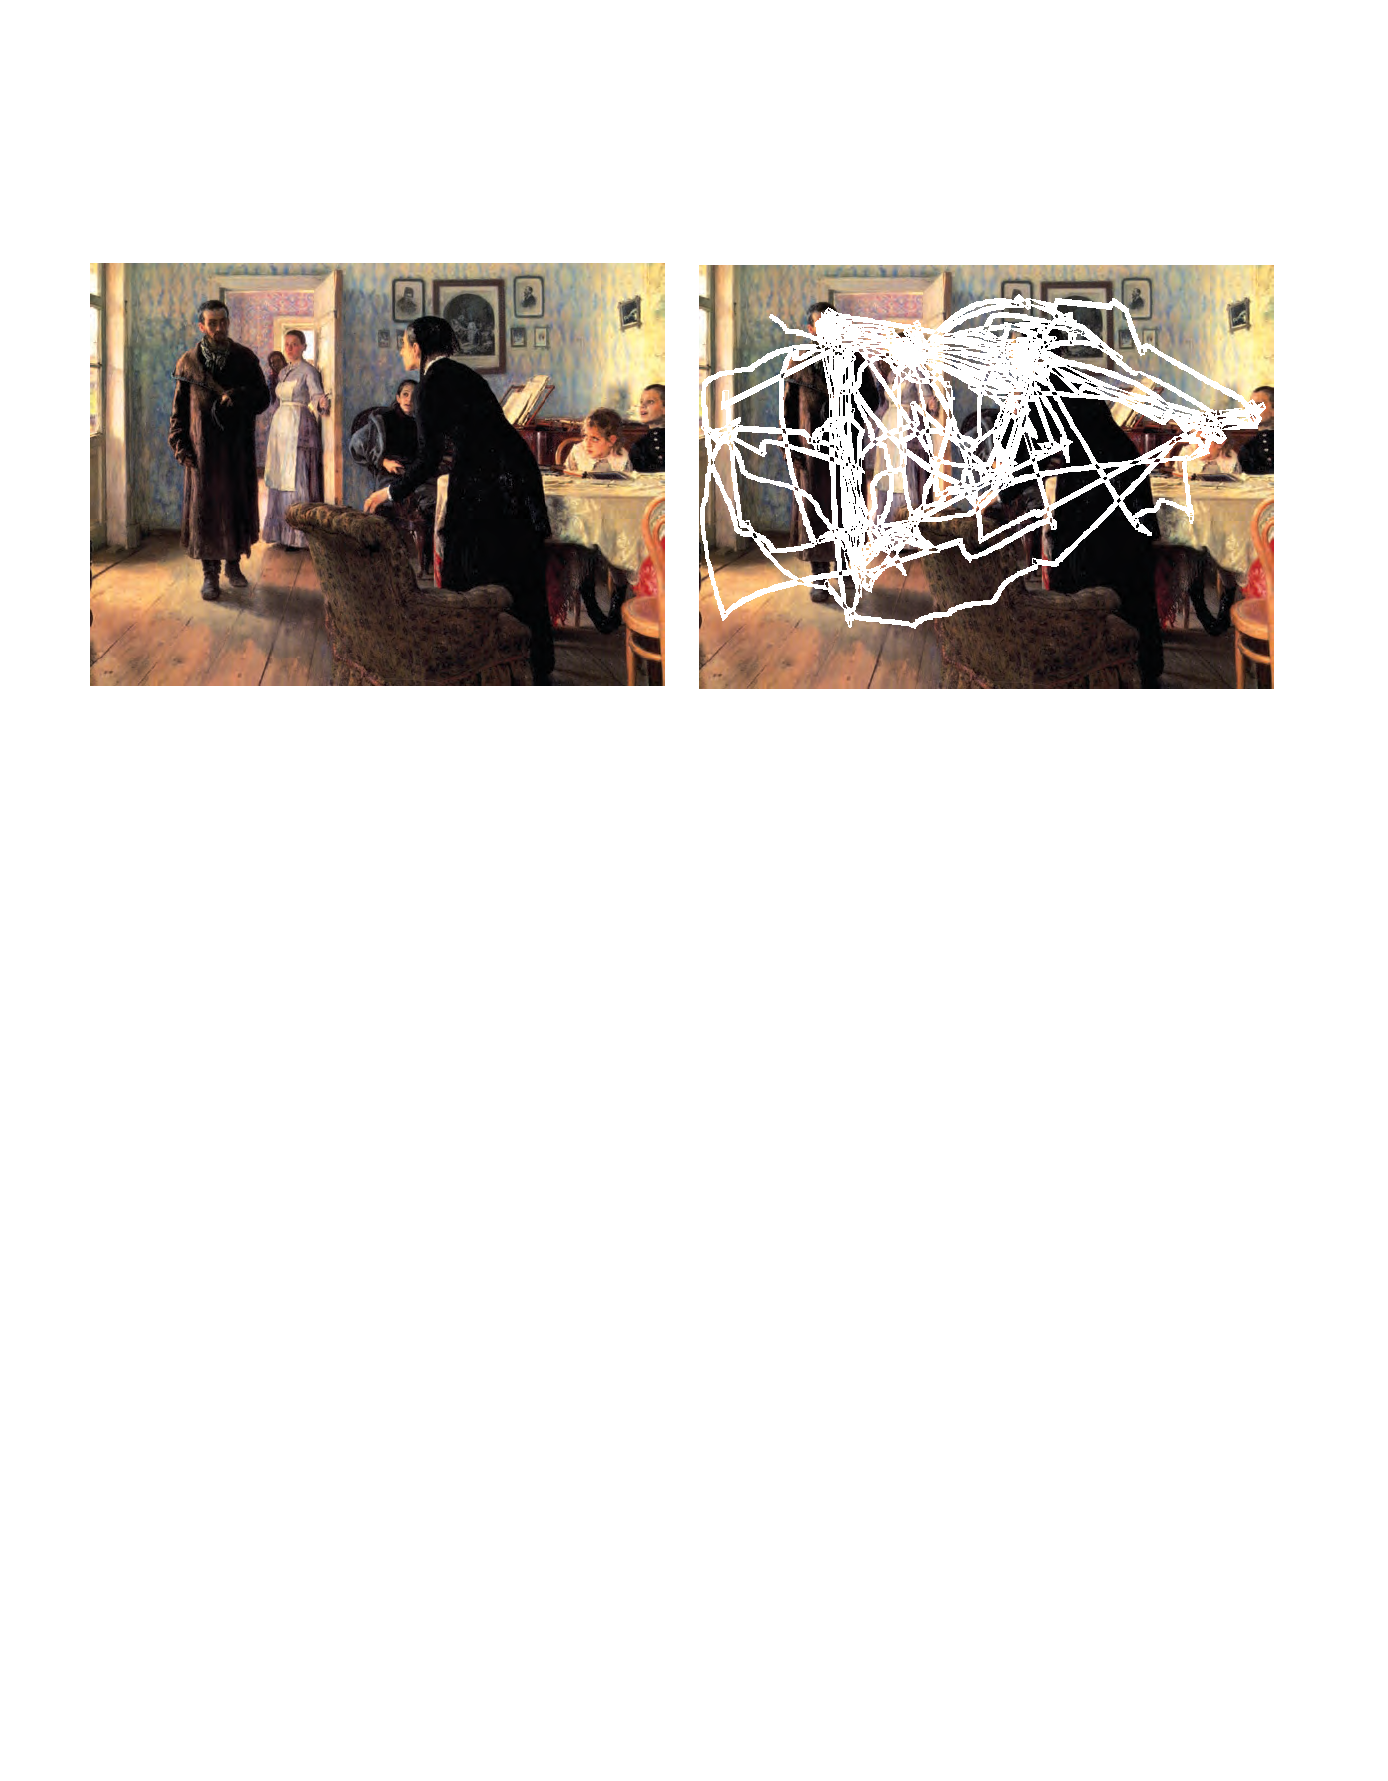
\includegraphics[width=0.8\linewidth]{chap25/fig_25_1}
	\caption{视觉过程中的眼球运动。
		受试者观看这幅画(\textit{伊利亚$\cdot$列宾}的《意外访客》)几分钟,对选定的注视点进行扫视,主要是面部。
		线条表示扫视,斑点表示注视点。}
	\label{fig:25_1}
\end{figure}


如图~\ref{fig:25_2}~所示,一个简单的实验室实验说明了大脑面临的生物学挑战。


\begin{figure}[htbp]
	\centering
	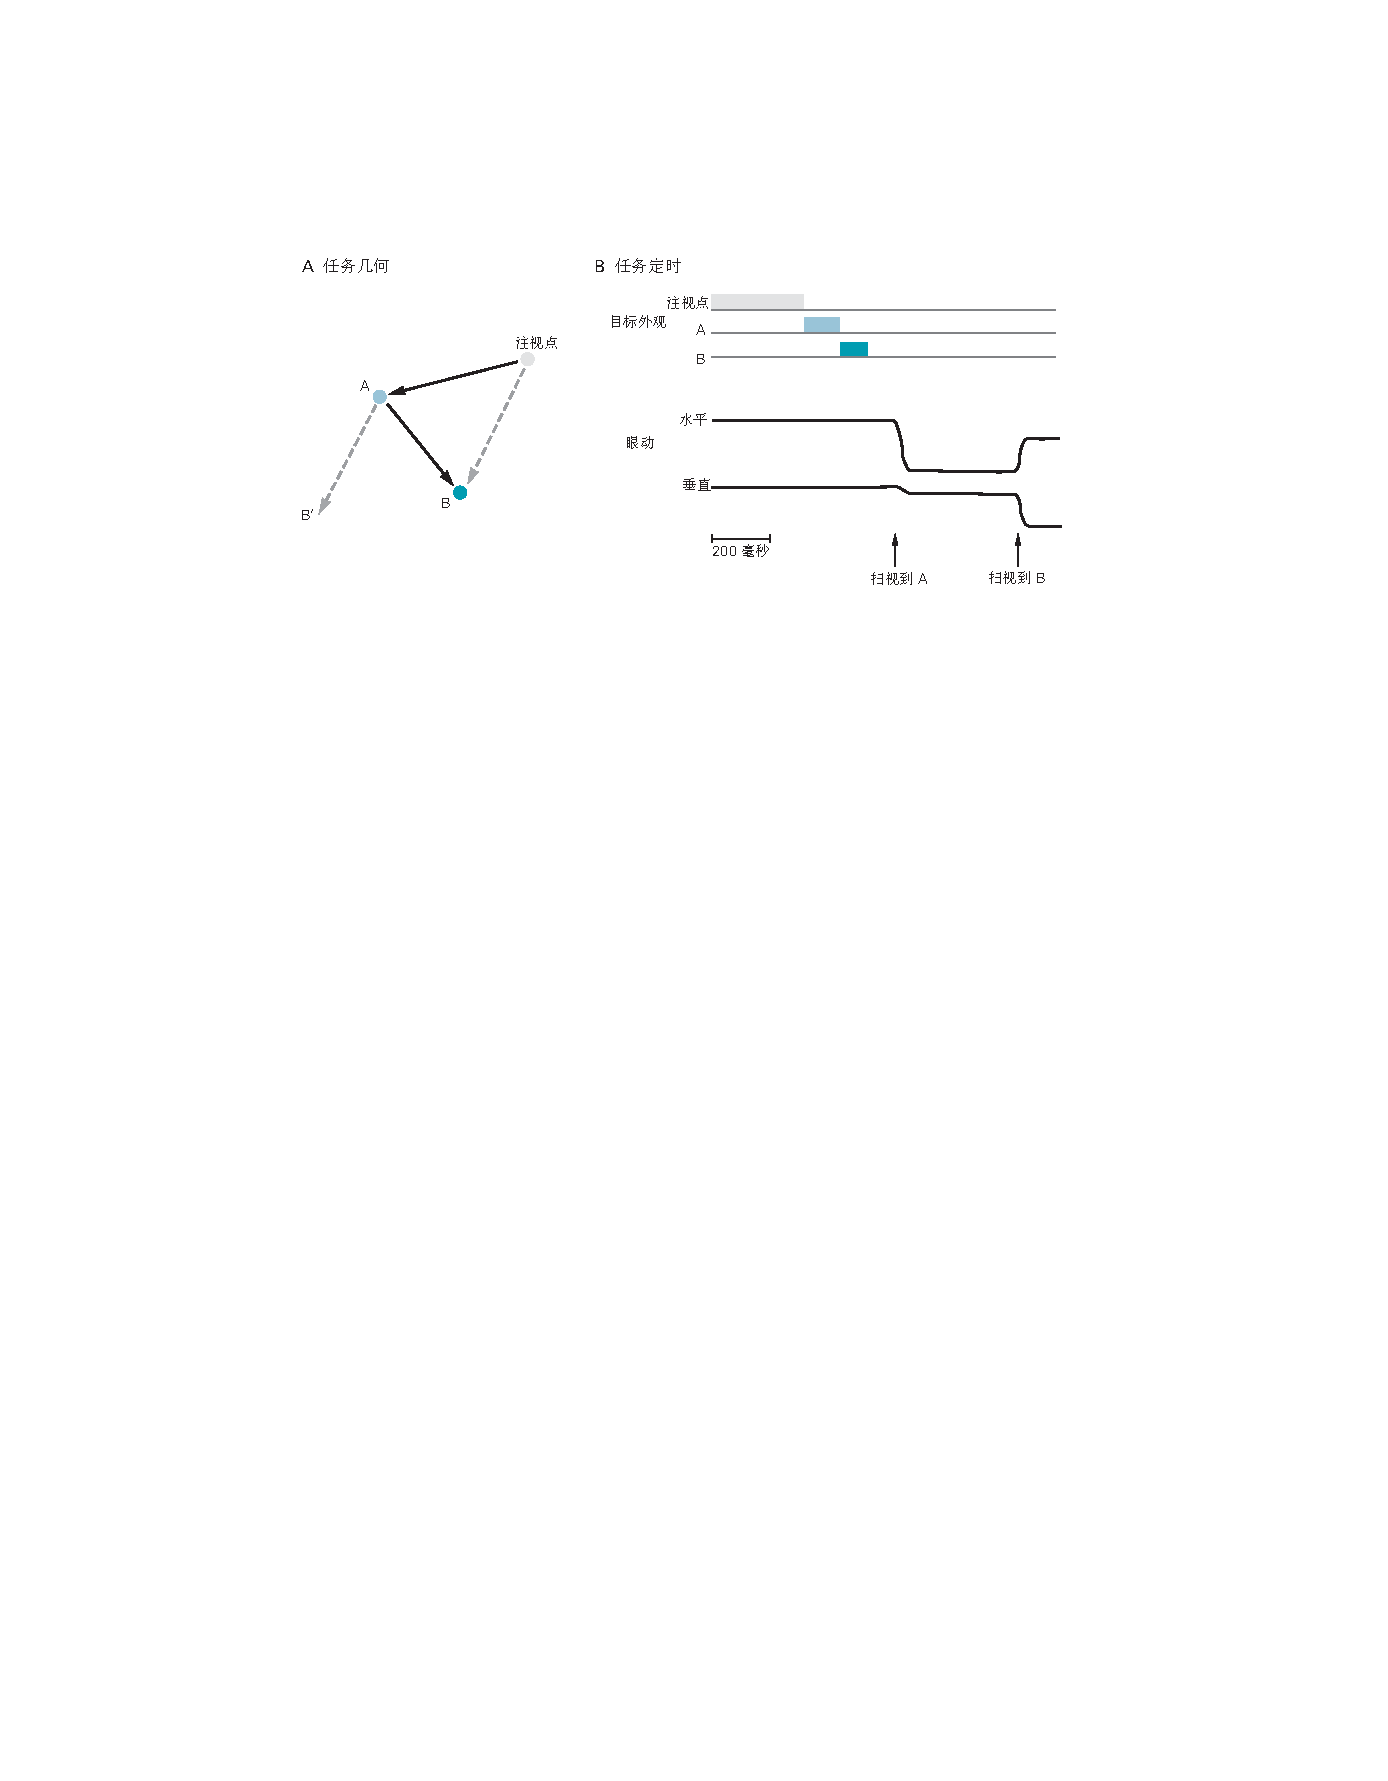
\includegraphics[width=0.9\linewidth]{chap25/fig_25_2}
	\caption{双步任务说明大脑如何在扫视期间稳定图像。
		\textbf{A.} 受试者首先注视一个消失的\textit{注视点},然后两个扫视目标 \textbf{A} 和 \textbf{B} 依次出现和消失,然后受试者才能进行扫视。
		第一个扫视(目标 A)很简单。
		视网膜向量(\textit{注视点}→A)和\textit{扫视}向量相同。
		% 中央凹还没到A?
		第一次扫视后,被试正在看A,视网膜向量为A→B',但猴子必须进行一次扫视,向量为A→B。
		大脑必须调整视网膜向量以补偿第一个扫视。
		\textbf{B.} 时序。
		上面的记录显示目标出现的时间(彩色条)。}
	\label{fig:25_2}
\end{figure}



\subsection{复制扫视的运动指令到视觉系统}

对视觉稳定性背后的大脑机制的第一个洞察来自\textit{赫尔曼$\cdot$冯$\cdot$亥姆霍兹}在 19 世纪的观察。
他看到一名患者由于外直肌麻痹而无法将眼球水平地移向耳朵。
当患者尝试将视线转向自己的耳朵时,他的视觉世界会短暂地跳转到相反的方向,随后又回到原先注视的中心点。


\textit{亥姆霍兹}假设每个扫视的运动命令副本被馈送到视觉系统,以便可以调整视觉世界的表示以补偿眼球运动。
这种调整将导致视觉世界的稳定图像。
在 19 世纪,\textit{亥姆霍兹}称这样的副本为“努力感”,而在 20 世纪,它被命名为\textit{传出副本}或\textit{伴随发送}。


\textit{伴随发送}解决了双步扫视的问题。
为了使\textit{伴随发送}影响眼球运动的视觉感知,运动信息必须影响视觉神经元的活动。
当猴子进行扫视时,顶叶皮层、额叶视区、纹状体视觉皮层和上丘中的神经元就会发生这种情况。
每个\textit{扫视}都可以被认为是一个具有两个维度的向量:方向和振幅。
尽管每次扫视后的视网膜图像都不同,但大脑可以使用每次扫视的向量从视网膜图像序列中重建整个视觉场景。


可以在单个细胞的水平上看到\textit{伴随发送}。
对恒河猴(一种动眼神经和视觉系统类似于人类的动物)的生理学研究阐明了这个问题。
每次猴子进行扫视时,因为当前不在\textit{侧顶叶}神经元的感受野中的刺激,所以无法激发神经元,如果即将发生的扫视将刺激带入感受野,则会激发神经元,甚至在扫视发生之前(图~\ref{fig:25_3})。
因此,即将发生的\textit{扫视}的\textit{伴随发送}会影响顶叶神经元的视觉反应。


\begin{figure}[htbp]
	\centering
	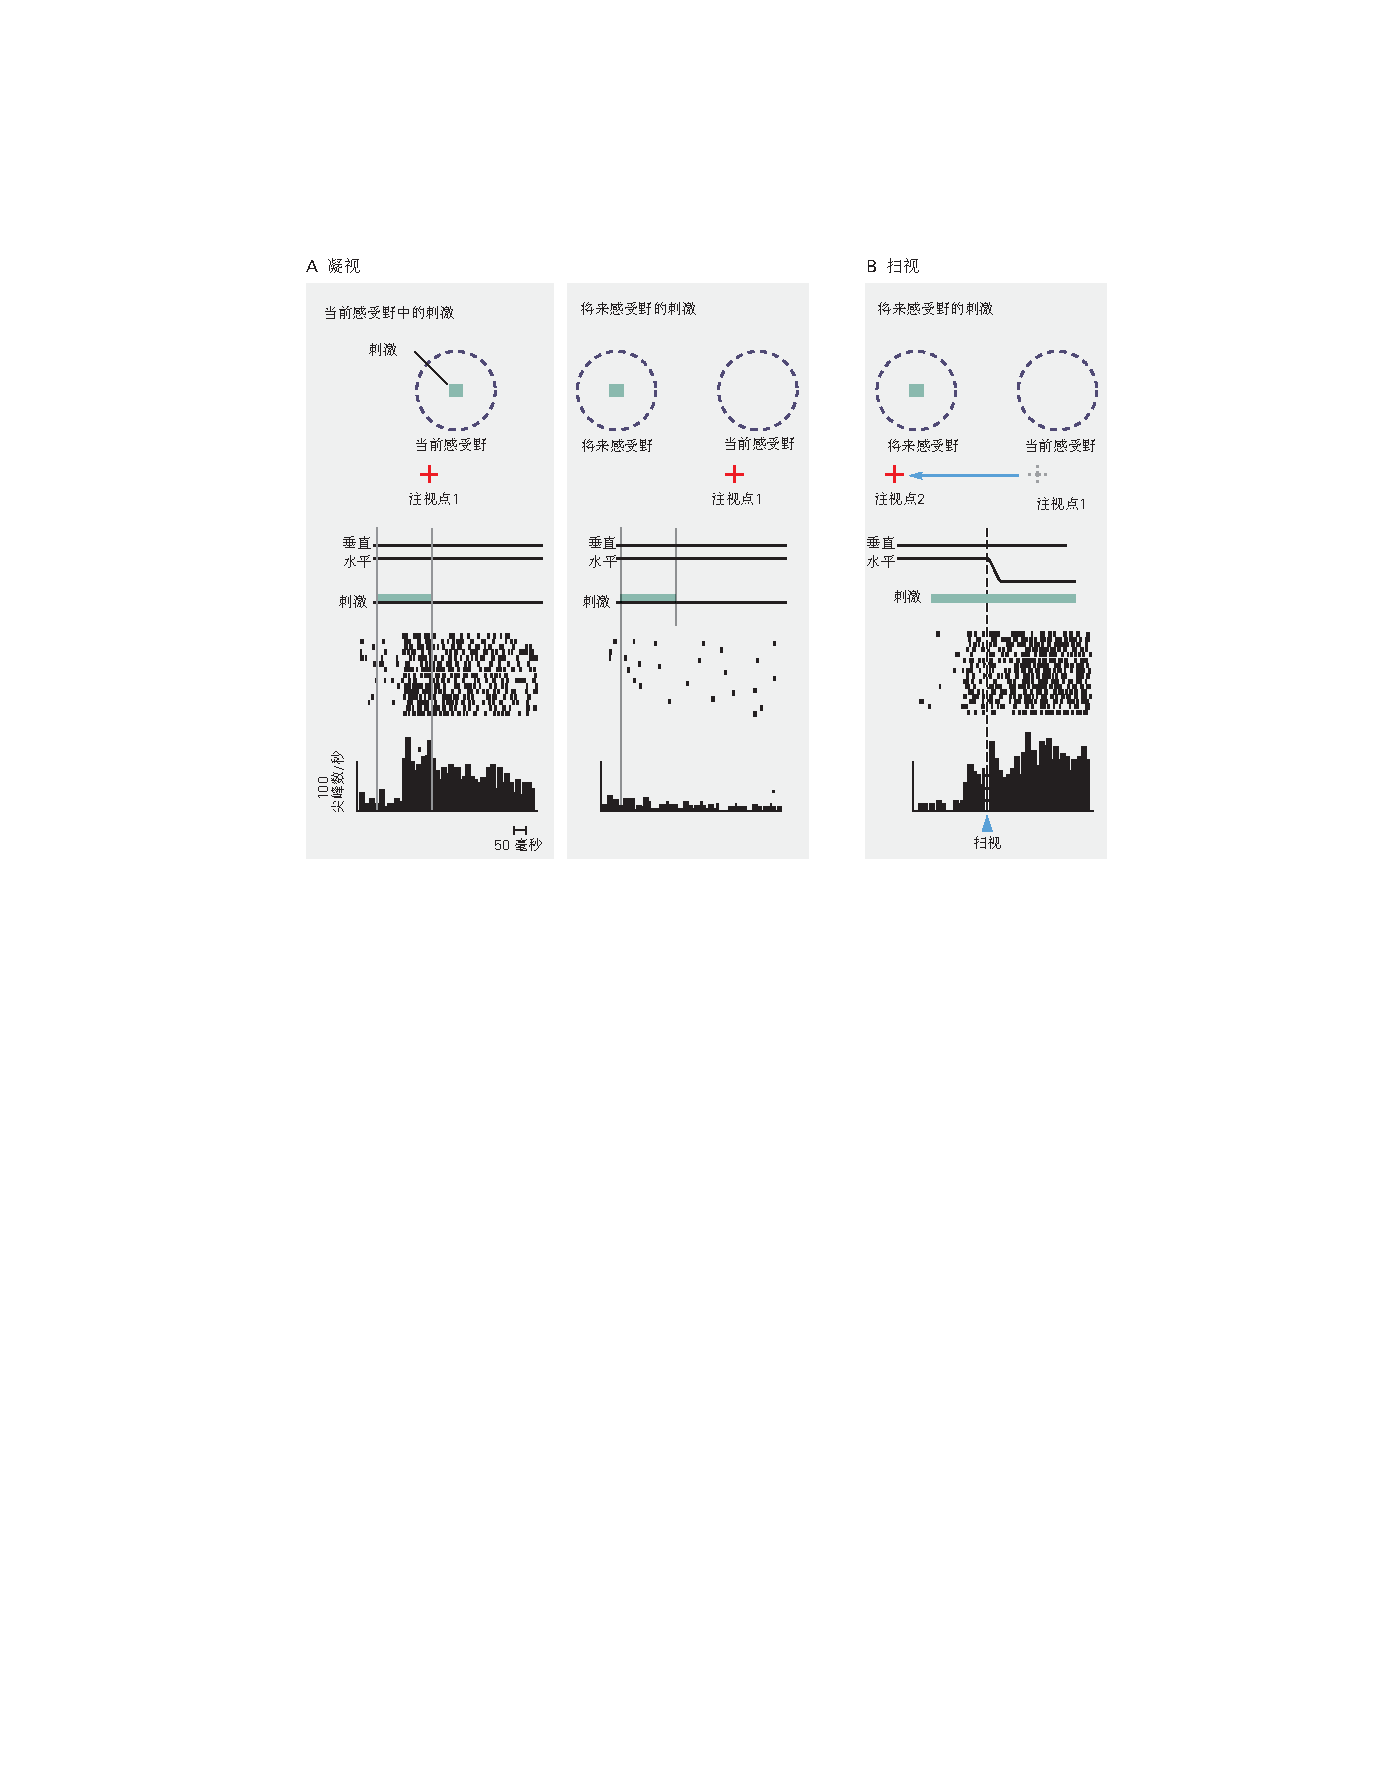
\includegraphics[width=1.0\linewidth]{chap25/fig_25_3}
	\caption{重新映射猴子顶叶皮层视觉神经元的感受野与扫视眼球运动\cite{duhamel1992updating}。
		\textbf{A.} 左:猴子\textit{注视点},并且细胞对\textit{当前感受野}中突然出现的与任务无关的刺激做出反应。
		连续试验在刺激出现时同步。
		右图:猴子看着 \textit{注视点}1,细胞对\textit{未来感受野}中闪现的刺激没有反应。
		\textbf{B.} 猴子从 \textit{注视点}1 到 \textit{注视点}2 进行扫视,这会将细胞的感受野带到\textit{未来感受野}中的刺激上。
		现在细胞甚至在\textit{扫视}开始之前就开始放电,这意味着\textit{扫视}计划的\textit{伴随发送}重新映射了细胞响应的视网膜区域。}
	\label{fig:25_3}
\end{figure}


% This transient remapping of
这种感受野的瞬态重新映射解释了受试者如何执行双步任务。
考虑图~\ref{fig:25_2}A~中的图表。
任务从猴子将目光对准\textit{注视点}开始。
在猴子进行第一次扫视后,视网膜向量 A→B' 不再对进行 A→B 扫视有用。
然而,\textit{注视点}→A 扫视重新映射描述向量 A→B 的细胞活动,因此它对视网膜位置的目标 B 做出反应,当猴子看\textit{注视点}时,该位置不在其感受野内。
在许多皮层和皮层下区域发现重映射,包括\textit{侧顶叶}、\textit{额叶视区}、\textit{内顶叶内区}、上丘中间层和前纹状体区 V4、V3a 和 V2。
正如我们将看到的,重新映射有助于扫视时的视觉感知和视觉引导运动的准确性。


这提出的第一个问题是:大脑如何获得它反馈给视觉系统的扫视向量?
我们从数十年的研究中了解到,向量的运动指令在中脑顶部的上丘中得到体现(第~\ref{chap:chap35}~章)。
上丘中的每个神经元都被调整到给定向量的\textit{扫视},这样神经元共同提供所有可能\textit{扫视}的向量图。
上丘的失活会影响猴子进行\textit{扫视}的能力。
对上丘进行的电刺激会引起刺激部位神经元所描述的向量\textit{扫视}。 
但这提供的是实际驱动眼睛的向量,而不是通知关于扫视向量的感知的向量。
用于移动眼睛的向量信息如何可用于不移动眼睛还需要有关其移动方式的信息的大脑过程?


由于在上丘中已经确定了移动眼球的向量,因此可以合理地预期这也可能是\textit{伴随发送}的来源。
它的确是。
上丘既有产生\textit{扫视}的下行通路,也有通往大脑皮层的上行通路,可以携带即将发生的运动的\textit{伴随发送}(图~\ref{fig:25_4})。
通往大脑皮层的通路通过丘脑,所有内部信息和几乎所有外部信息都通过丘脑到达大脑皮层。


\begin{figure}[htbp]
	\centering
	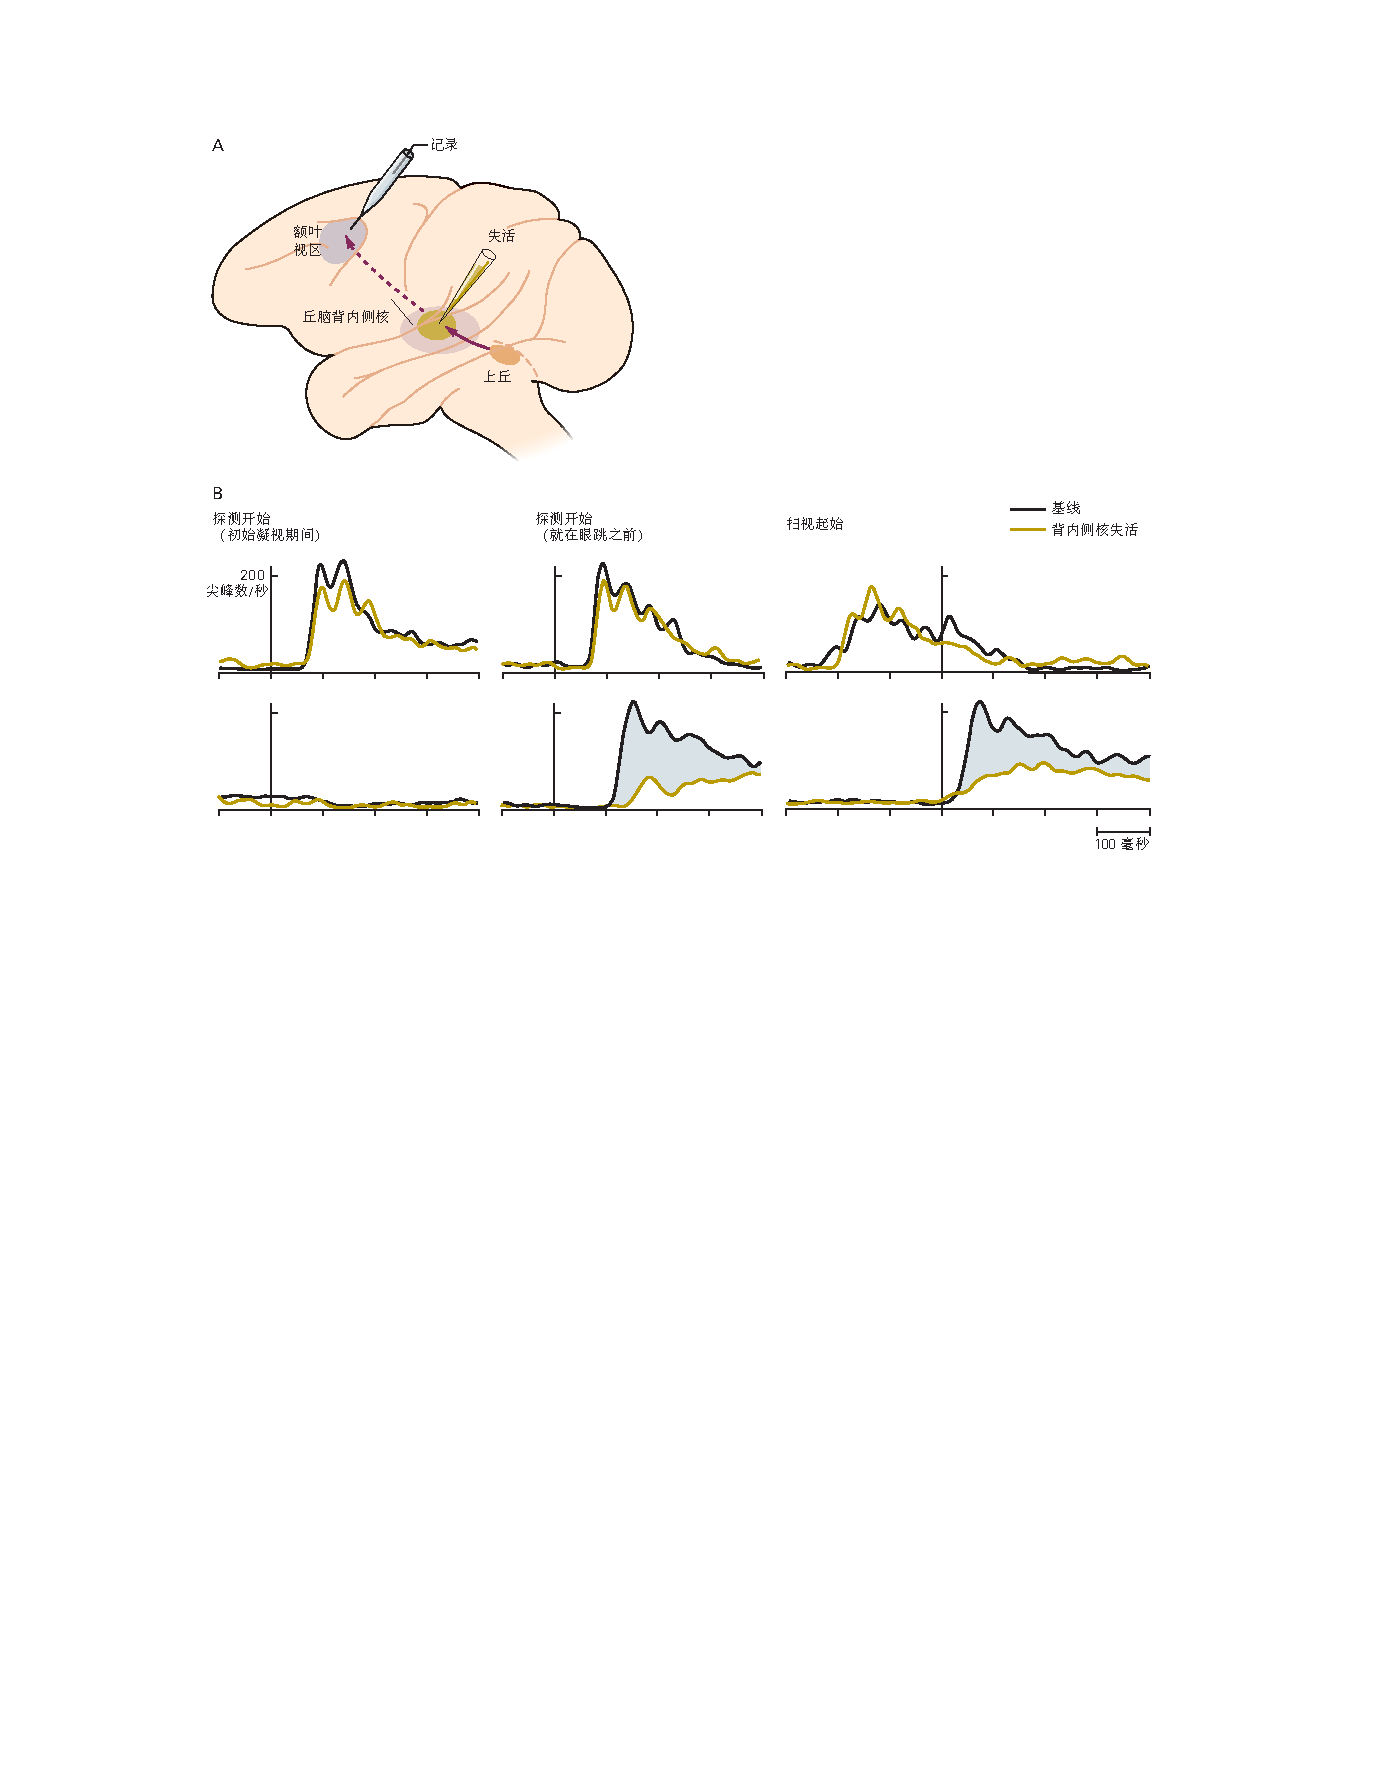
\includegraphics[width=1.0\linewidth]{chap25/fig_25_4}
	\caption{扫视运动程序的\textit{伴随发送}会导致在扫视之额叶视区神经元的感受野位置发生变化\cite{sommer2008brain}。
		\textbf{A.} \textit{伴随发送}的一种可能途径起源于上丘中产生\textit{扫视}的神经元,穿过丘脑的内侧背核,并终止于额叶皮层的\textit{额叶视区}。
		\textbf{B.} 当\textit{背内侧核}失活时,额叶视区神经元对细胞当前感受野中刺激探针的反应不受影响(上部记录),而对未来刺激的反应(后-扫视)感受野严重受损(记录较低)。
		这一结果表明,扫视运动程序的\textit{伴随发送}指导神经元感受野特性的转变。}
	\label{fig:25_4}
\end{figure}


% The motor signal in the thalamus
丘脑中的运动信号不一定是\textit{伴随发送};
它也可能是简单地通过大脑皮层的运动命令。
然而情况并非如此,因为丘脑中这条通路的失活不会改变\textit{扫视}的幅度和方向。
它不是在驱动扫视,更有可能是\textit{伴随发送}。
丘脑通路失活后,猴子无法准确执行双步任务的第二次扫视。
此外,失活会破坏前面描述的感受野重新映射(图~\ref{fig:25_3}B)。
因为破坏\textit{伴随发送}会破坏感受野重新映射和眼球运动的行为补偿,\textit{伴随发送}可能对于解决动作的空间准确性问题至关重要。


为了确定\textit{伴随发送}是否也提供了允许视觉系统感知在扫视之前出现的物体位置的信息,猴子被训练以指出它认为它的眼球在扫视结束时指向的位置。
我们可以测量运动系统移动眼睛的位置,但我们想知道的是猴子对每次扫视时眼睛方向变化的感知。
这可以使用\textit{海纳$\cdot$多伊贝尔}及其同事为人类开发并适用于猴子的任务来确定。
在此任务中,猴子注视一个注视点,然后扫视一个目标(图~\ref{fig:25_5}A)。
在扫视过程中,目标暂时消失;
当它再次出现时,它已被移至原始目标的左侧或右侧位置。
试验后,猴子向右或向左移动一根棒子以指示位移的方向(图~\ref{fig:25_5}A)。


\begin{figure}[htbp]
	\centering
	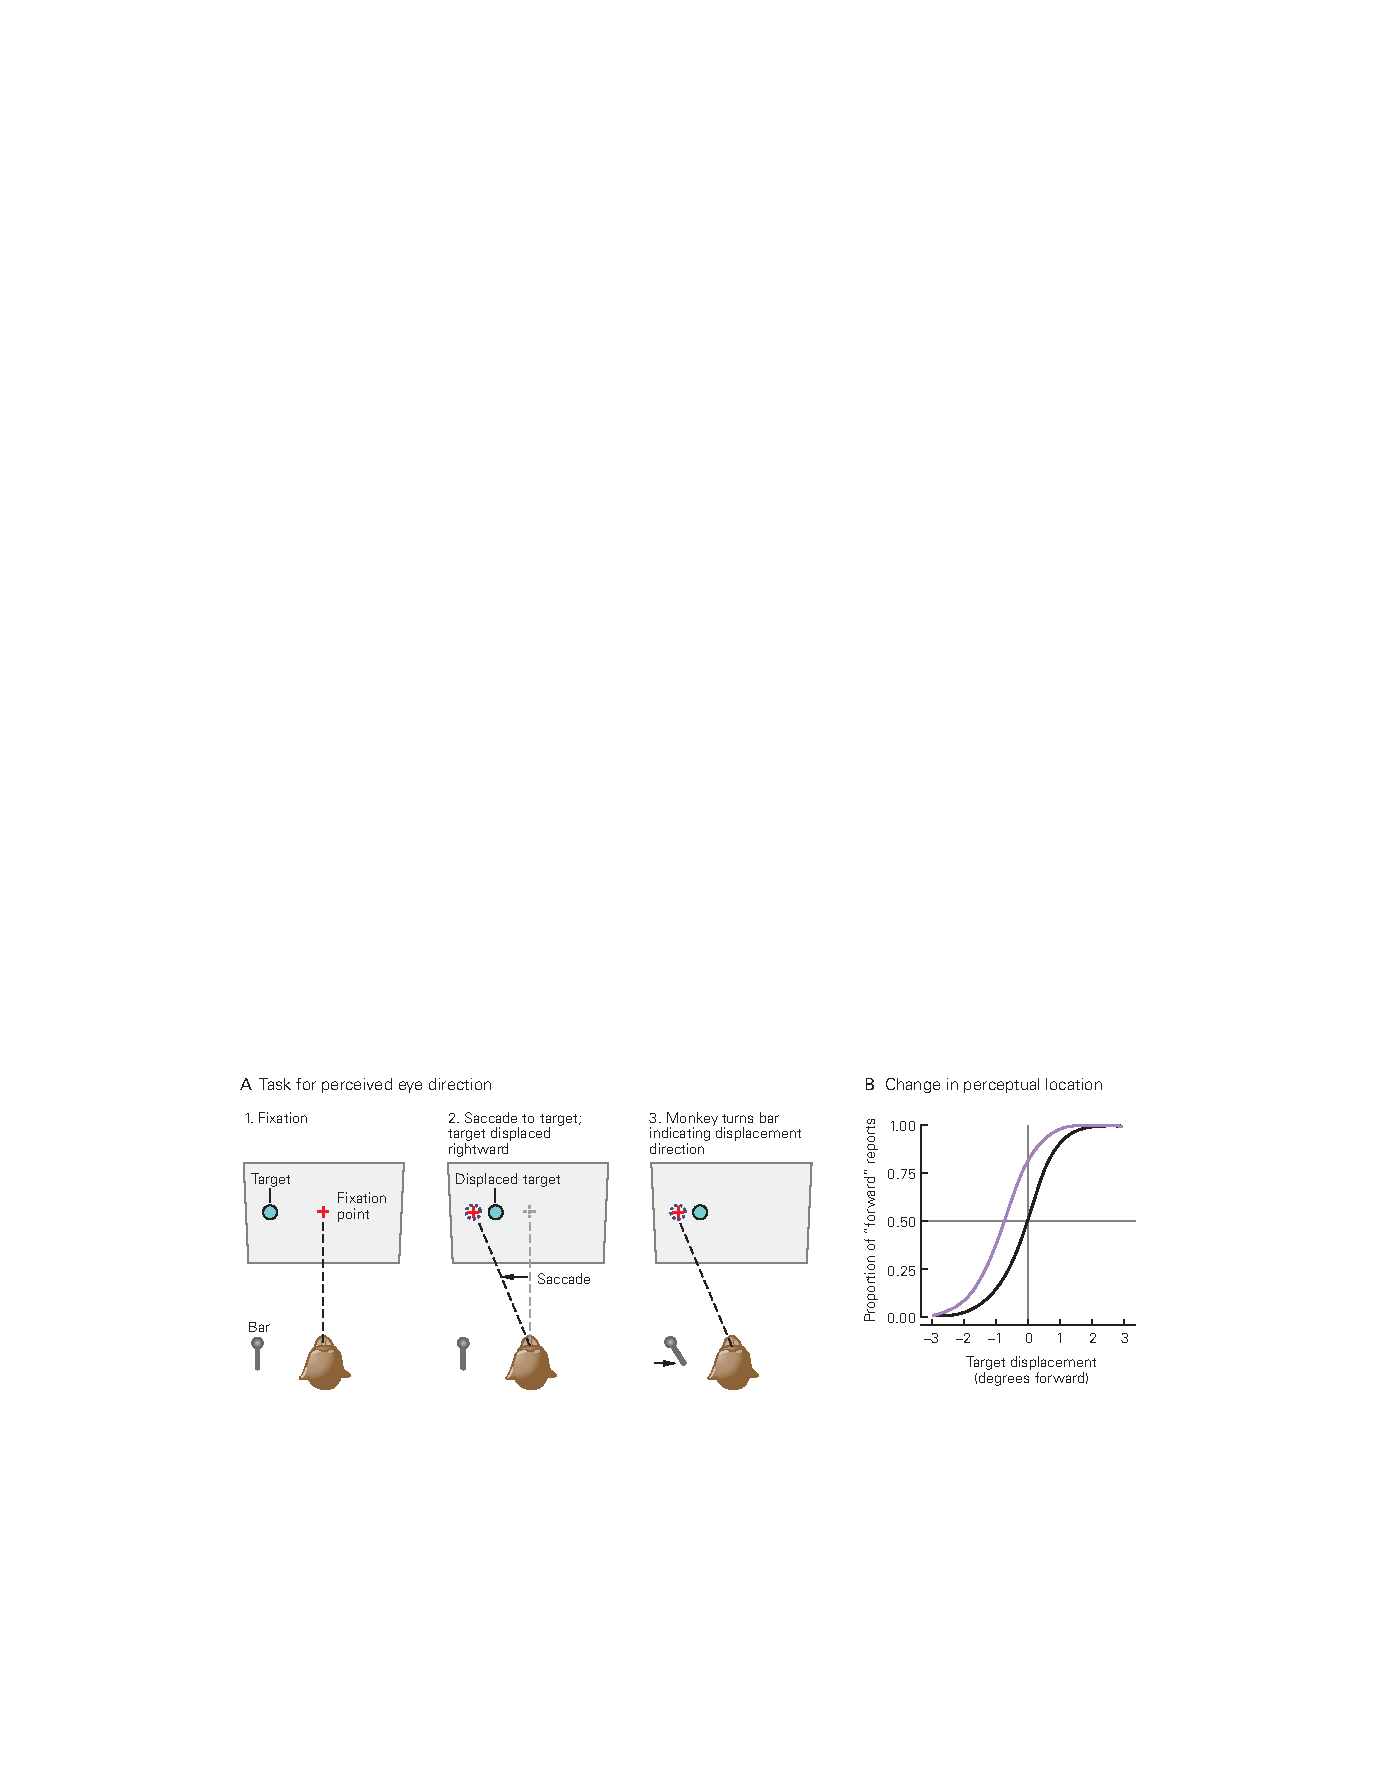
\includegraphics[width=1.0\linewidth]{chap25/fig_25_5}
	\caption{感知到的扫视方向随着\textit{伴随发送}的中断而改变。
		\textbf{A.} 在每次试验开始时,猴子都会在屏幕上注视一个目标(1)。
		当注视点关闭时,猴子会向目标扫视;
		在扫视期间,目标随机(最多 3°)向左或向右移动(2)。
		在扫视到原始目标后,猴子会收到一个奖励,用于在目标位移的方向上手动移动一个杆(3)。
		\textbf{B.} 丘脑内侧背核失活之前(黑色)和失活之后(紫色)的心理测量曲线,其中包含在上丘和额叶皮层之间的通路中进行\textit{伴随发送}的中继神经元。
		该曲线显示了每个目标位移(x 轴)的向前(在扫视方向)判断(y 轴)的比例。
		猴子没有感知到位移的扫视后目标位置被定义为\textit{感知零点}\cite{cavanaugh2016saccadic}。}
	\label{fig:25_5}
\end{figure}


在一系列试验中,猴子的反应被绘制成一条心理测量曲线(图~\ref{fig:25_5}B)。
此曲线显示与初始扫视相同(向前)或相反(向后)方向的实际眼内目标位移(水平轴),以及猴子报告它向前移动的频率(垂直轴)。
猴子的回应是,当目标向右倾斜 3° 时,目标已经向前移动了 100\%。
当目标向左移动 3° 时,猴子的反应是它从未向前移动过。
心理测量曲线上猴子以相同频率报告向前和向后位移的点(50\% 水平线)被视为\textit{感知零点}。
我们将此点作为猴子对原始目标位置的感知。
如果目标未被感知到移动,则它必须位于与扫视之前相同的位置;
在正常的猴子中,该点接近于零(图~\ref{fig:25_5}B)。


% We now have a corollary discharge
我们现在有一个\textit{伴随发送},可以为每个扫视提供向量,并为猴子提供一项任务,使我们能够确定它在扫视结束时感知目标的位置。
如果\textit{伴随发送}有助于猴子的感知,那么使\textit{伴随发送}失活应该会改变动物对目标位置的感知。
确实如此,图~\ref{fig:25_5}B~中的紫色曲线表示\textit{伴随发送}失活后的感知位置;
丘脑内侧背核失活后曲线向左移动。
结论是\textit{伴随发送}确实提供了扫视的向量,这是猴子能感知到目标已经移动所必须的。
对于每个\textit{扫视},\textit{伴随发送}信息提供了用于确定当前\textit{扫视}的幅度和方向的感知信息,并且它以机器般的精度每秒执行几次。


% The corollary discharge provides
\textit{伴随发送}提供了\textit{扫视}之前可用的向量信息,但它不是唯一的信息来源。
在扫视发生后,必须评估另外两种类型的信息:\textit{视觉提示}和眼肌本体感觉。
\textit{视觉提示}不太可能成为所描述感知实验中的一个因素(图~\ref{fig:25_5}),因为实验是在完全黑暗中进行的,除了从非常暗淡的注视点和扫视目标散射的光。
然而,在光线下,\textit{视觉提示}会是一个因素吗?
事实上,在光线下重复这个实验并没有提高猴子的判断力,反而使它的判断能力变差。


动眼神经本体感觉不太可能在扫视结束时提供向量信息,因为平均而言,失活前和失活过程中扫视的指标不会改变,因此几乎没有理由期望肌肉本体感觉会发生变化。
此外,虽然\textit{伴随发送}至少在\textit{扫视}前 100 毫秒开始,但来自动眼神经本体感觉的神经元活动在\textit{扫视}后约 150 毫秒到达\textit{侧顶叶}。
正如我们将在下一节中看到的,本体感觉在知觉中的作用可能是在扫视结束很久之后提供信息。


% Finally, there is a second
最后,\textit{扫视}还会产生第二种潜在的视觉干扰:\textit{扫视}扫过视网膜的视觉场景时会出现模糊。
然而,这种模糊是看不见的,因为在每次扫视时,许多视觉区域的神经元活动都受到抑制。
这种所谓的扫视抑制首先出现在上丘,随后出现在丘脑和初级视觉皮层以外的视觉皮层区域。


% A corollary discharge contributes to this
\textit{伴随发送}有助于这种神经元活动抑制,因为即使在完全黑暗(无视觉)和眼球运动受阻(无本体感觉)的情况下也会发生抑制。
抑制也可以通过视觉遮蔽产生,当一种刺激减少了对后续或先前刺激的感知时,就会发生这种情况。
如果扫视在完全黑暗中开始,然后一个物体在扫视结束前闪过并熄灭,则在扫视期间可以看到模糊。
如果在扫视之后闪过一个掩模,模糊就会被抑制。
在初级视觉皮层的神经元中可以清楚地看到这种\textit{遮蔽效应}的相关性。
由\textit{伴随发送}产生的抑制相对较弱,但存在于所有\textit{扫视}中;
来自视觉遮蔽的效果要强得多,但仅存在于光线中。



\subsection{动眼神经本体感觉有助于精确的空间感知和行为}

\textit{查尔斯$\cdot$谢林顿}提出,大脑补偿眼睛移动的方式是直接测量眼睛在眼眶中的位置,并根据位置变化调整视觉信号。
\textit{理查德$\cdot$安德森}和\textit{弗农$\cdot$芒卡斯尔}发现,具有视网膜感受野的顶叶视觉神经元的反应是由眼睛在眼眶中的位置以一种称为\textit{增益场}的方式线性调制(图~\ref{fig:25_6})。
从这个关系中,可以很容易地计算出物体在以头部为中心(头颅)坐标中的位置。


\begin{figure}[htbp]
	\centering
	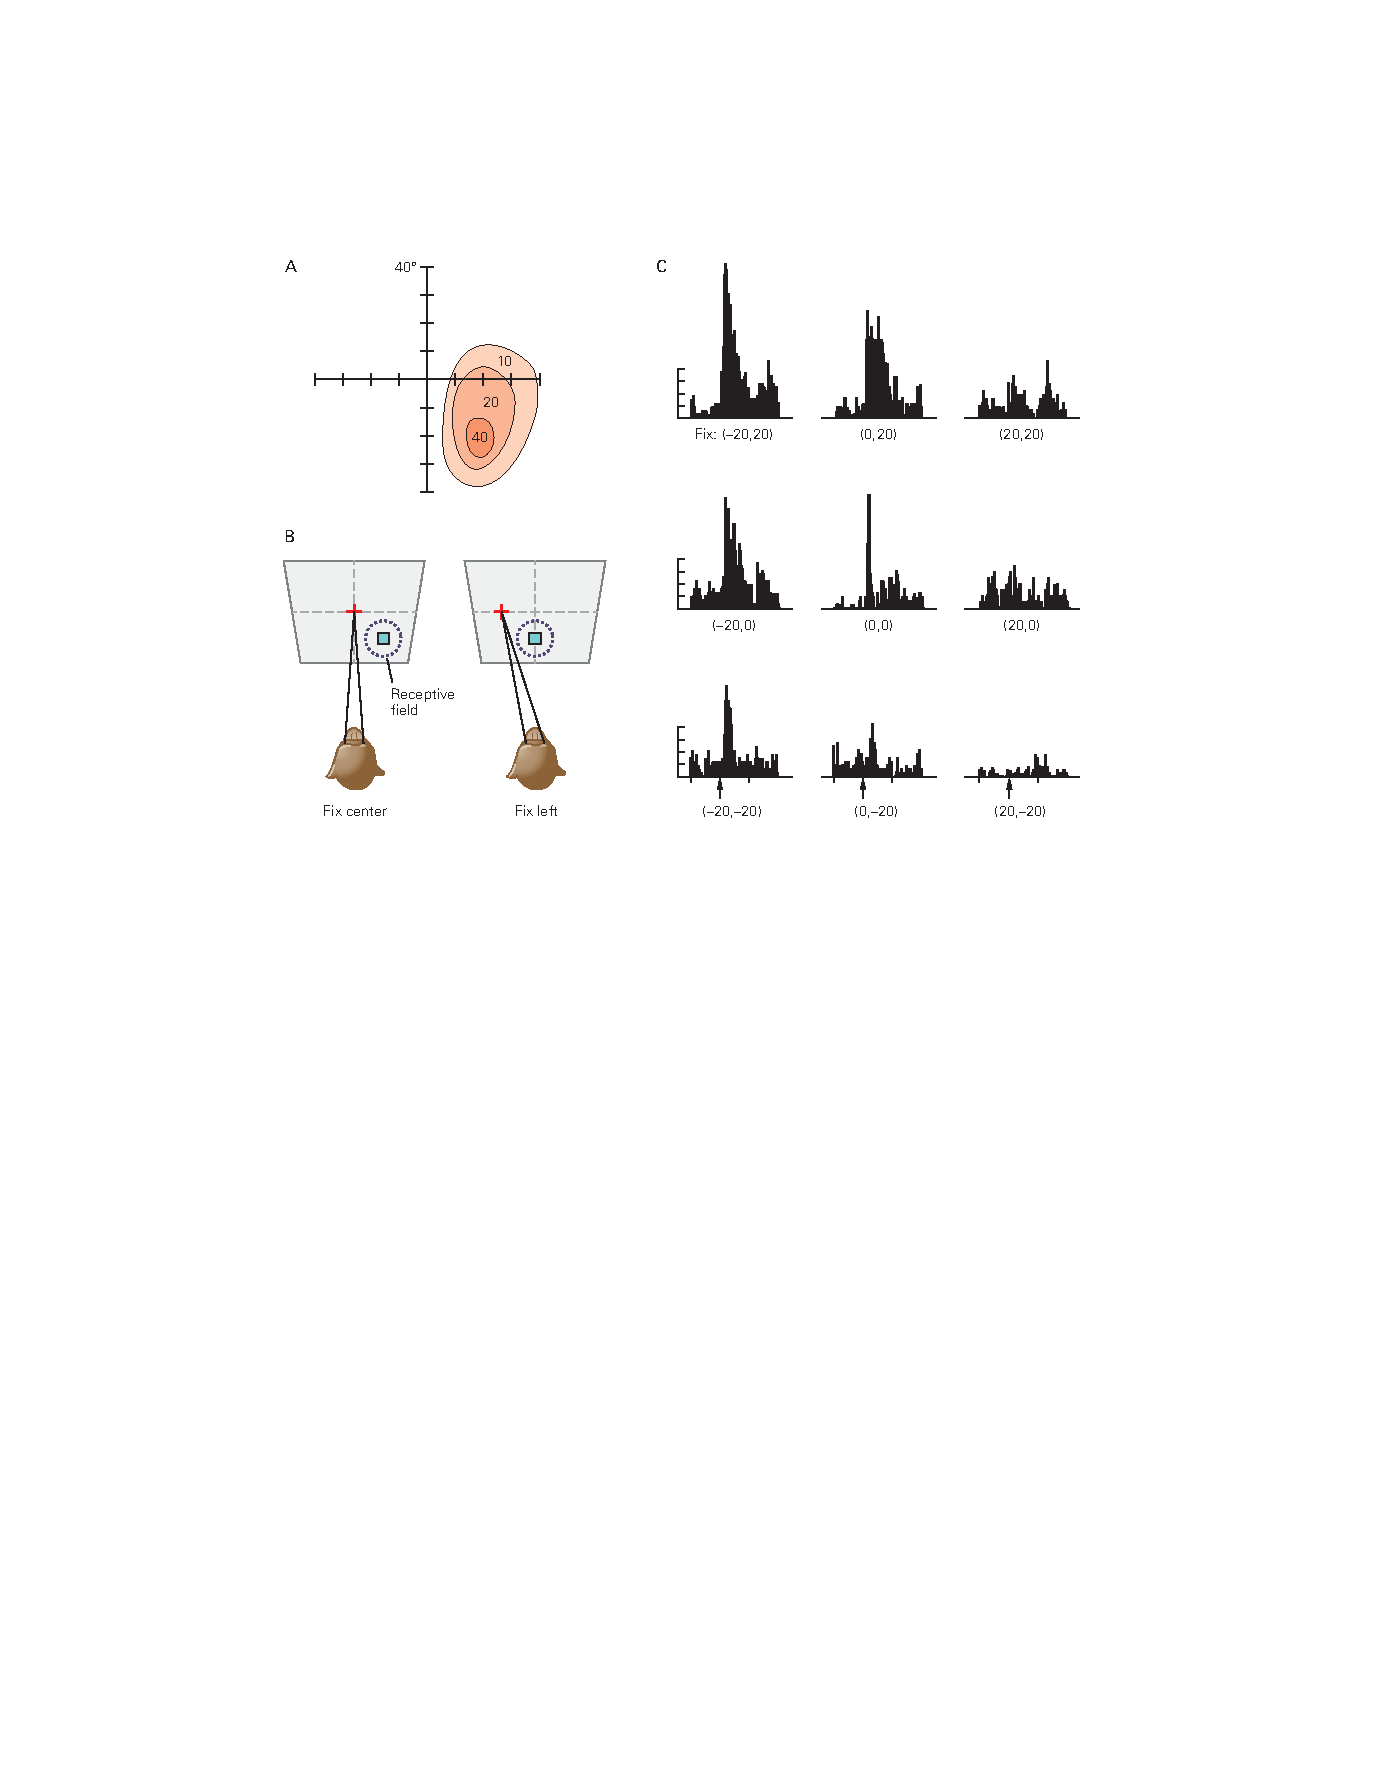
\includegraphics[width=1.0\linewidth]{chap25/fig_25_6}
	\caption{眼睛在眼眶中的位置会影响顶叶视觉神经元对视网膜感受野的反应。
		\textbf{A.} 相对于中央凹的感受野。等高线图表示不同空间位置的尖峰率。
		数字是每个轮廓在最大位置的每秒峰值。
		\textbf{B.} 感受野随眼睛在空间移动。
		在左边,猴子正在注视屏幕的中心。
		在右侧,同一只猴子注视着中心左侧 20°。
		对于 C 中的记录,刺激(蓝色方块)始终呈现在感受野的中心。
		\textbf{C.} 在感受野的最佳位置对刺激的反应随着眼睛在眼眶中的位置而变化,从猴子注视(-20°、20°)时的最大值到猴子注视(20°,−20°)时的最小值。
		箭头表示刺激闪光的开始。
		试验时间为 1.5 秒;
		纵坐标,25 个尖峰/格\cite{andersen1985encoding}。}
	\label{fig:25_6}
\end{figure}


产生\textit{增益场}的眼睛位置信号从何而来?
它可能来自眼睛位置的\textit{伴随发送},也可能来自本体感受机制。
人眼肌肉有两种结构可能有助于动眼神经本体感觉:
肌梭和肌腱柱体,或栅栏末端,这是一种眼睛特有的结构。
3a 区是骨骼肌纺锤体投射到的体感皮层区域,它代表了眼睛的位置,由对侧眼眶的本体感受器产生(图~\ref{fig:25_7})。


\begin{figure}[htbp]
	\centering
	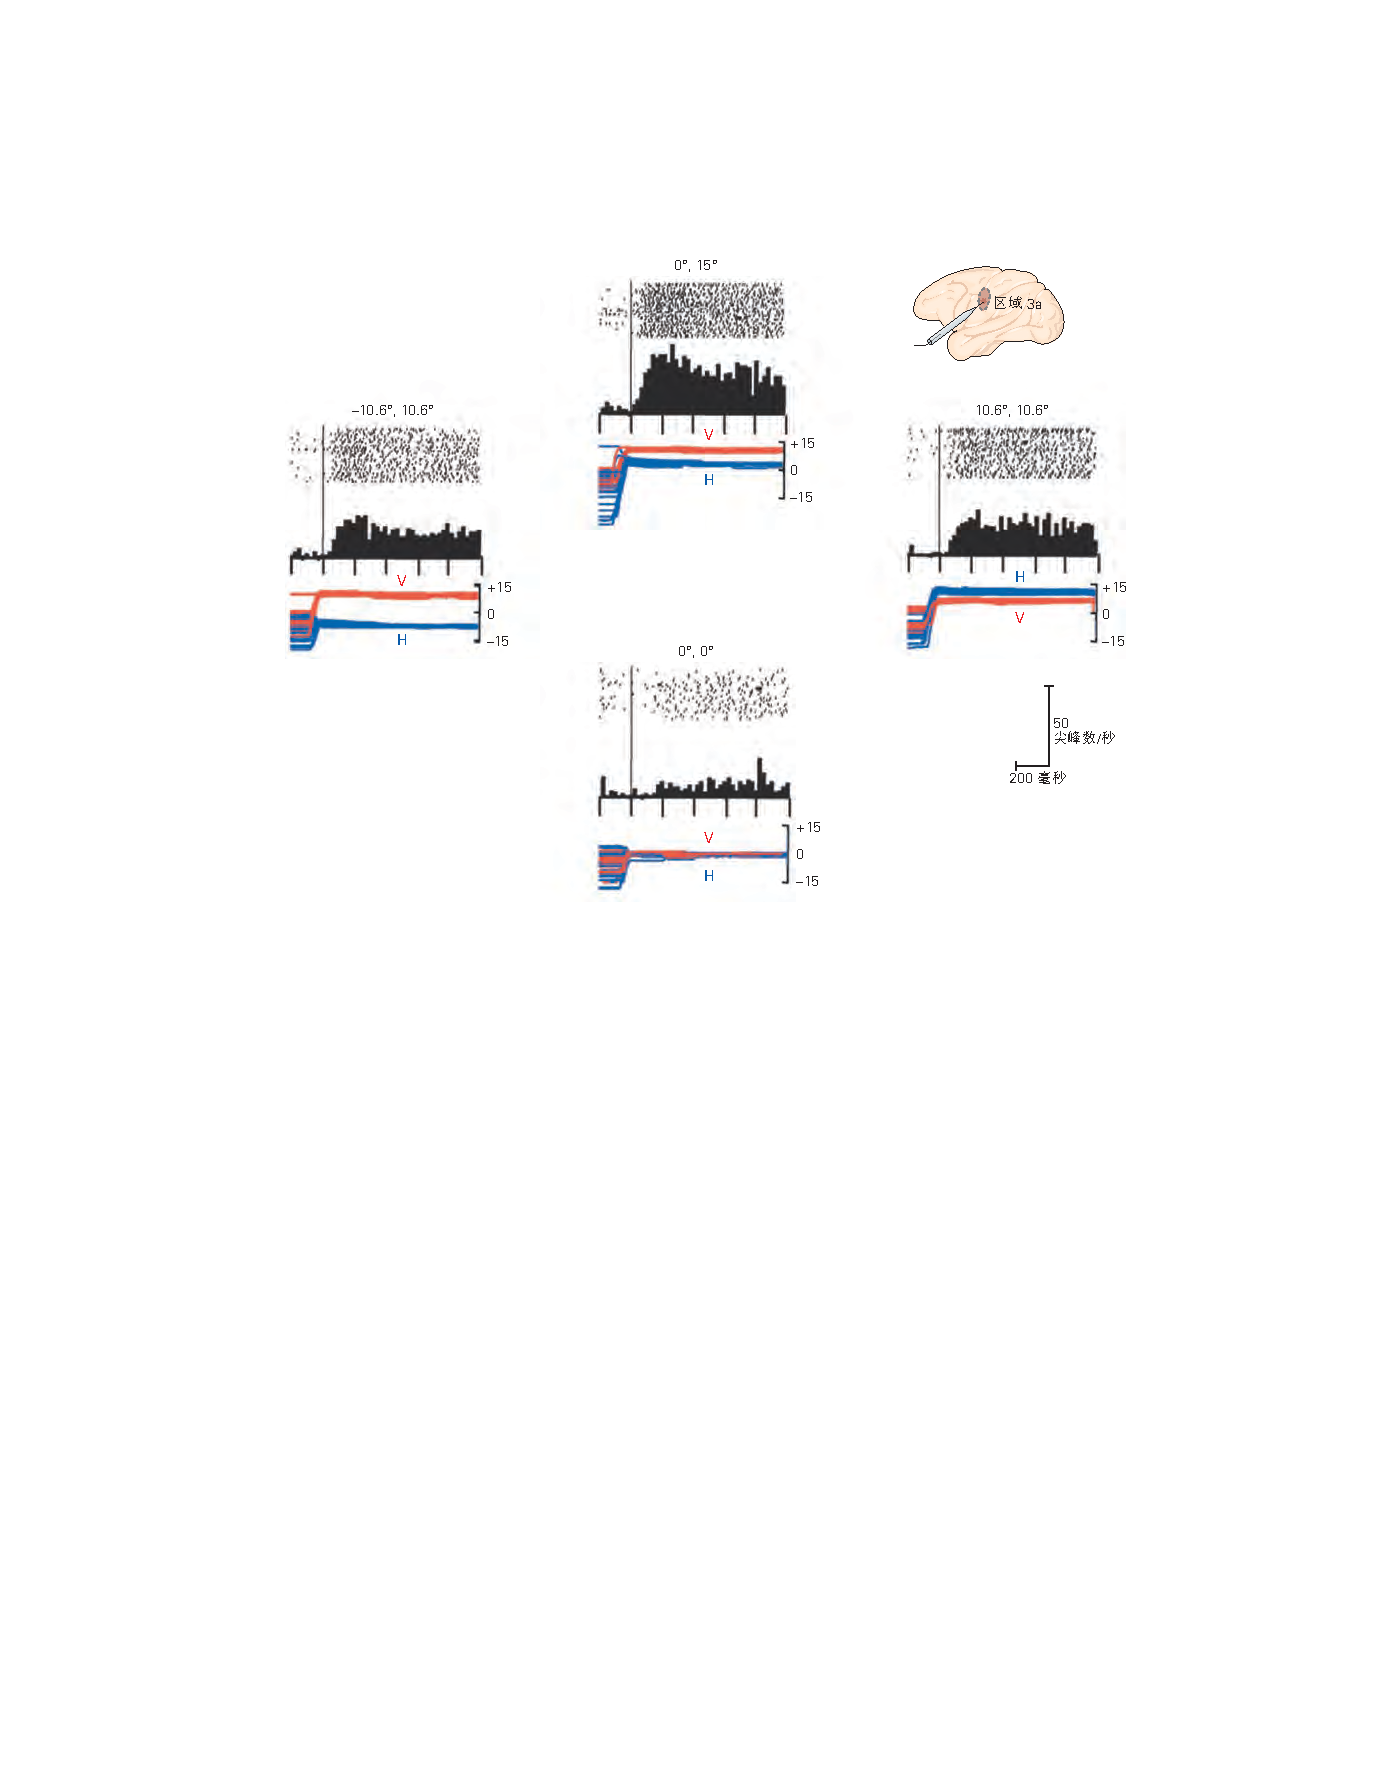
\includegraphics[width=1.0\linewidth]{chap25/fig_25_7}
	\caption{体感皮层区 3a 中的眼睛位置神经元。
		每个面板显示\textit{水平}和\textit{垂直}眼睛位置以及猴子对每个光栅上方指示的眼睛位置进行扫视后神经元的活动。
		当眼睛处于 0°、15° 时,神经元的反应比在 0°、0° 时要快得多。}
	\label{fig:25_7}
\end{figure}


然而,眼睛位置的本体感受测量滞后于眼睛位置的变化 60 毫秒,并且在扫视后的 150 毫秒内,增益场调节视觉反应,就好像猴子仍在看扫视前的目标一样,在\textit{伴随发送}已经很久之后重新映射视觉响应。
因此,产生增益场的眼睛位置信号可能来自本体感受机制。
大脑有可能使用两种机制计算在眼球运动之前出现的物体的空间位置:
快速的\textit{伴随发送}和缓慢但比\textit{伴随发送}更准确的本体感受信号。
本体感受信号也可用于校准\textit{伴随发送}。



\section{视觉审查是由注意力和唤醒回路驱动的}

在 19 世纪,\textit{威廉$\cdot$詹姆斯}将注意力描述为“头脑以清晰而生动的形式占据似乎同时可能出现的多个目标或多个思路中的一个。
它意味着从某些事情中退缩,以便有效地处理其他事情。” 
\textit{詹姆斯}接着描述了两种不同的注意力:“它要么是被动的、反射性的、非自愿的、毫不费力的,要么是主动的、自愿的。
在被动的直接感官注意中,刺激是一种感官印象,要么非常强烈、大量,要么突然……大的东西、明亮的东西、移动的东西……血液。”


您在阅读本页时对本页的关注是自愿关注的一个例子。
如果一道亮光突然闪过,你的注意力可能会不由自主地从页面上移开。
在注意力焦点之外发生的视觉场景中的巨大变化通常会被忽略,直到主体将注意力转移到它们上,这种现象被称为\textit{变化盲}(图~\ref{fig:25_8})。


\begin{figure}[htbp]
	\centering
	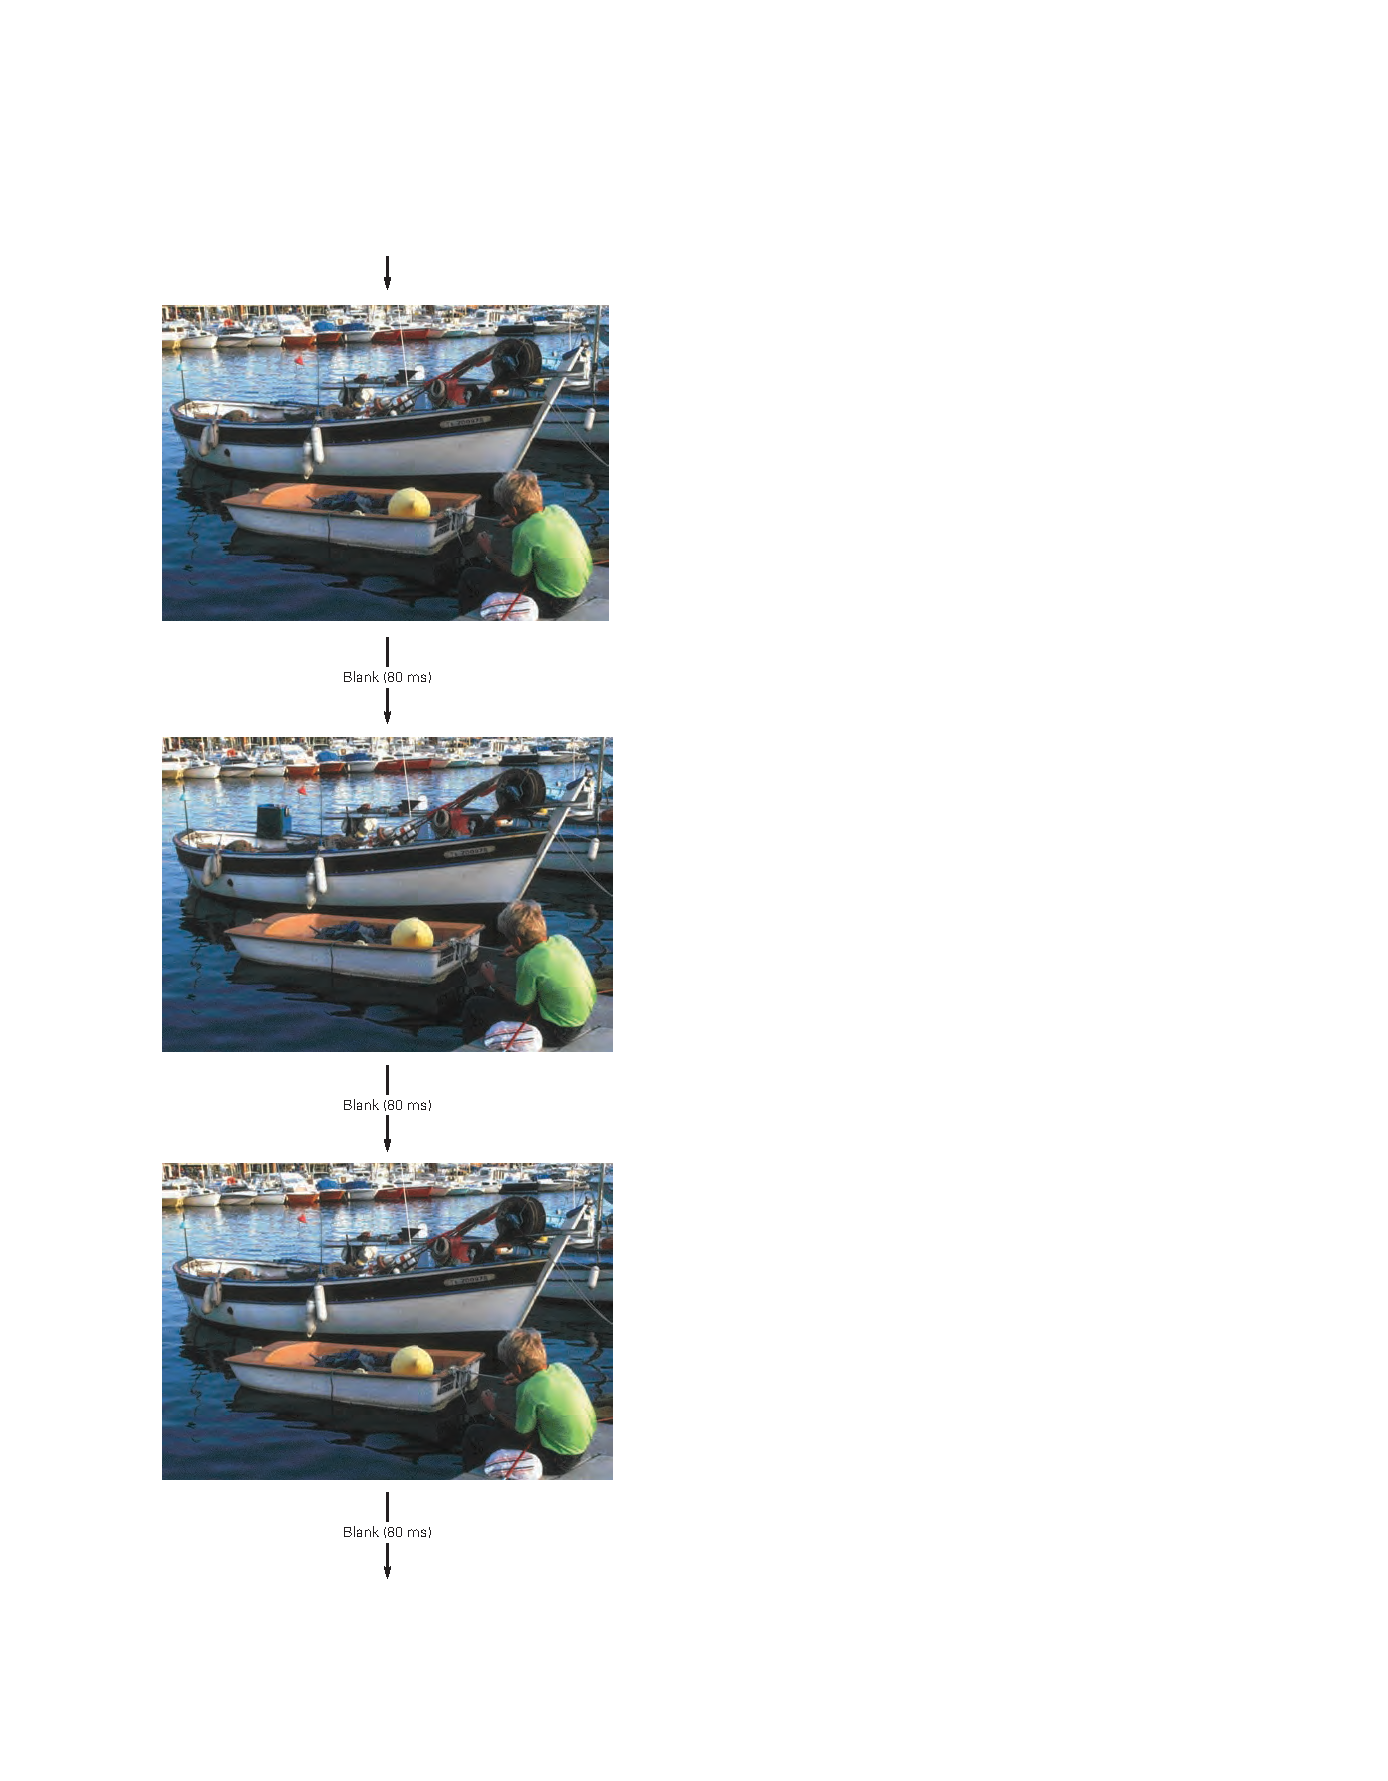
\includegraphics[width=0.53\linewidth]{chap25/fig_25_8}
	\caption{\textit{变化盲}。
		在\textit{变化盲}测试中,先显示一张图片,然后是 80 毫秒的空白屏幕,然后是第二张图片,另一张空白屏幕,然后重复该循环(左)。
		受试者被要求报告场景发生了什么变化。
		% 第二章图的床头有个箱子
		尽管两张照片之间存在实质性差异,但大多数观察者需要多次重复才能发现差异。}
	\label{fig:25_8}
\end{figure}


有意的注意与扫视的眼球运动密切相关,因为中央凹的视锥细胞阵列比周边视网膜密集得多(第~\ref{chap:chap17}~章),并且将中央凹移至注意的目标允许进行比周边视觉可能进行的更细粒度的分析。
选择空间中的一个点的注意力,无论是否伴随\textit{扫视},都称为空间注意力。
搜索特定类型的目标,例如红色和绿色 Q 中的红色 O,涉及第二种注意力,即特征注意力:在搜索中,你忽略绿色字母而只关注红色字母。


有意和无意的注意力会缩短反应时间并使视觉感知更加敏感。
这种提高的灵敏度包括以较低对比度检测物体并忽略靠近关注物体的干扰物的能力。
行为无关的提示(例如闪光)突然出现,减少了对 300 毫秒后在同一位置出现测试刺激的反应时间。
相反,当提示远离测试刺激出现时,反应时间会增加。
闪光会不自觉地引起人们对其位置的注意,从而加速对测试刺激的视觉反应。
类似地,当受试者计划对视野的特定部分进行扫视时,可以检测到任何物体的对比度阈值会通过提示提高 50\%。


临床研究长期以来一直将顶叶与视觉注意力联系起来。
右侧顶叶病变的患者视野正常。
当在简单的视觉环境中用单一刺激研究他们的视觉感知时,他们的反应是正常的。
然而,当呈现更复杂的视觉环境时,左右视觉半场都有物体,这些患者倾向于报告左半场(病变对侧)的内容少于右半场(病变同侧)。
这种缺陷,称为忽视(第~\ref{chap:chap59}~章),是因为注意力集中在病变同侧的视觉半场上。
即使患者只接受两种刺激,每个半视野一个,他们也报告说只看到同侧半视野的刺激。
当注意力集中在受影响半野的一个刺激上,而第二个刺激出现在未受影响的半野时,患者没有能力将注意力转移到新的刺激上,即使从眼睛到纹状体和前纹状体皮层的感觉通路 完好无损。


这种对对侧视觉半视野的忽视延伸到对单个物体的对侧一半的忽视(图~\ref{fig:25_9})。
右顶叶缺损患者通常难以再现绘图。
例如,当被要求画一个时钟时,他们可能会将所有数字强制放在钟面的右侧,或者当被要求平分一条线时,他们可能会将中线放在该线实际中心的右侧。


\begin{figure}[htbp]
	\centering
	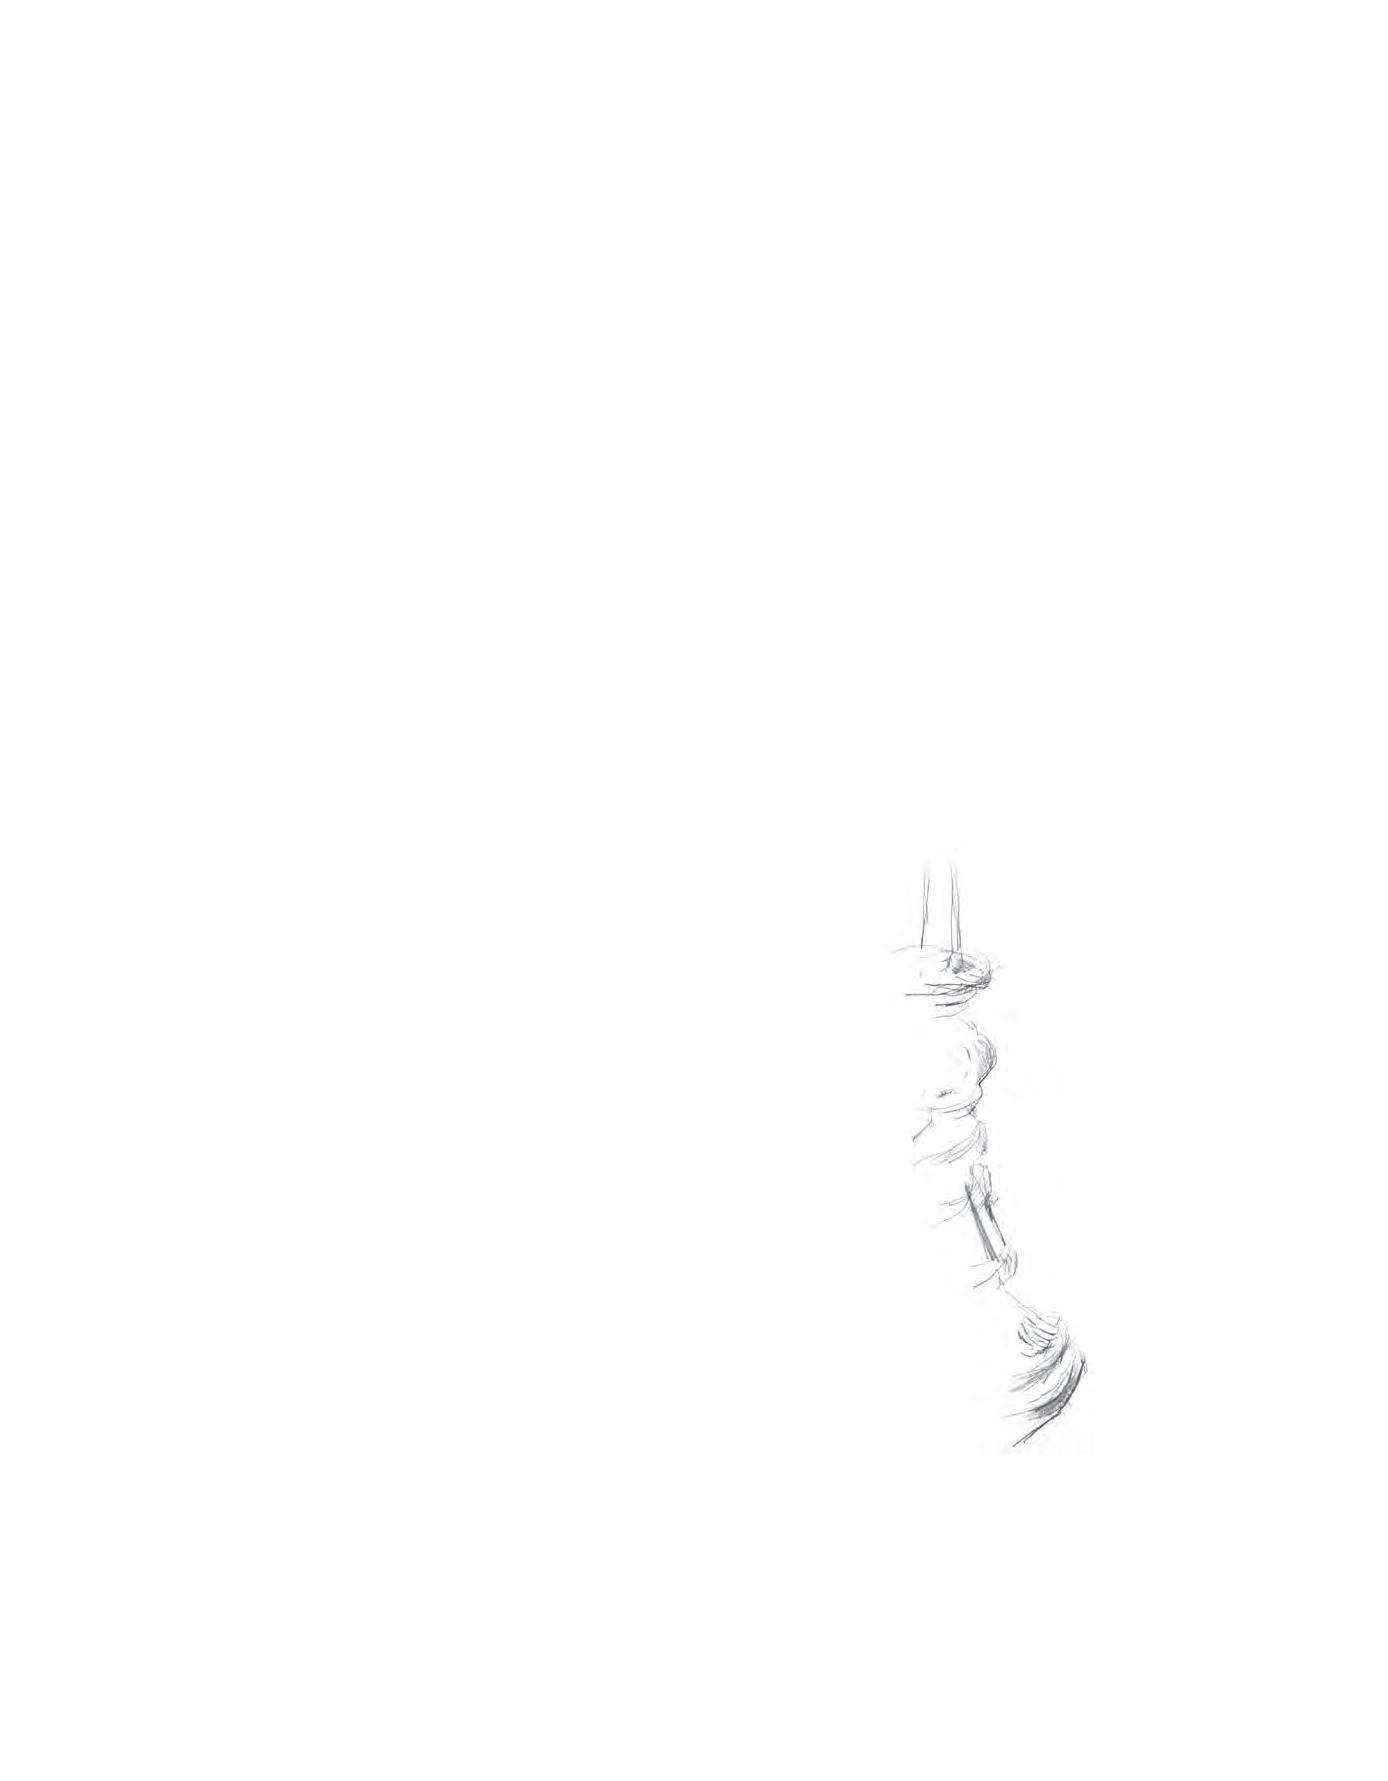
\includegraphics[width=0.4\linewidth]{chap25/fig_25_9}
	\caption{右顶叶损伤患者绘制的烛台图。
		病人忽略了烛台的左侧,只画了它的右半部分。}
	\label{fig:25_9}
\end{figure}


注意选择的过程在猴子的单个顶叶神经元水平上是显而易见的。
\textit{侧顶叶}神经元对视觉刺激的反应不仅取决于刺激的物理特性,还取决于它对猴子的重要性。
因此,对行为无关刺激的反应远小于对任何引起注意事件的反应,例如在感受野中突然出现视觉刺激或计划对神经元的感受野进行扫视。


虽然\textit{侧顶叶}的神经元共同代表整个视觉半场,但任何时刻活跃的神经元仅代表半场中的重要目标,即视野的\textit{优先级图}。
外侧顶叶内区域充当许多不同信号的汇合点:扫视规划、突然刺激发作和搜索特征的认知方面。


一个物体引起的神经元反应的绝对值本身并不能决定该动物是否正在注意该物体。
当一只猴子计划对视野中的刺激进行扫视时,注意力集中在扫视的目标上,而扫视计划引发的活动位于\textit{优先级图}的顶部。
然而,如果明亮的光线出现在视野的其他地方,注意力就会不由自主地被吸引到明亮的光线上,这会比扫视计划唤起更多的神经元活动。
因此,只能通过检查整个\textit{优先级图}并选择其峰值来识别注意力点;
它不能仅通过监测任何一点的活动来识别(方框~\ref{box:25_1})。


\begin{proposition}[顶叶皮层的\textit{优先级图}] \label{box:25_1}
	
	\quad \quad 猴子顶内外侧区域的神经元只代表那些对猴子具有潜在重要性的物体,即视野的\textit{优先级图}。
	这种对行为重要物体的选择性可以通过猴子的神经元记录来证明,而猴子在一系列稳定的物体上进行眼动。
	
	\quad \quad 视觉世界中稳定的物体很少成为人们关注的目标。
	与大脑的大多数其他视觉中心一样,在顶内外侧区域,神经元感受野是视网膜变性的;
	也就是说,它们是相对于凝视中心来定义的。
	当猴子扫描视野时,每次眼球运动时,固定物体都会进入和离开神经元的感受野,而不会干扰猴子的注意力(图~\ref{fig:25_10})。
	
	\quad \quad 视觉刺激的突然出现会不由自主地引起注意。
	当与任务无关的光在顶内外侧神经元的感受野中闪烁时,该细胞反应迅速(图~\ref{fig:25_11}A)。
	相反,当眼球运动将稳定的、与任务无关的刺激带入神经元的感受野时,它几乎不会引起反应(图~\ref{fig:25_11}B)。
	
	\quad \quad 将稳定物体带入感受野的扫视可能会抑制视觉反应。
	事实并非如此。
	第二个实验使用了类似的阵列,只是在稳定阵列实验中,在扫视引起感受野的位置没有刺激。
	猴子固定,使阵列中没有任何成员在感受野中,然后与任务无关的刺激突然出现在感受野的接种后位置。
	现在,猴子向阵列的中心扫视,将最近出现的刺激带到感受野,细胞剧烈放电(图~\ref{fig:25_11}C)。
	当猴子做扫视动作时,两个阵列是相同的。
	然而,稳定的刺激可能是无人看管的,而最近闪现的刺激引起了人们的注意和更大的反应。
	当稳定的物体与动物当前的行为相关时,它们可以引起增强的反应。
	
	\quad \quad 一个稳定的目标在行为上也很重要。
	在这种情况下,当猴子必须注意由扫视带入感受野的稳定物体时,神经元会增加它们的放电速率(图~\ref{fig:25_12})。
	
\end{proposition}


\begin{figure}[htbp]
	\centering
	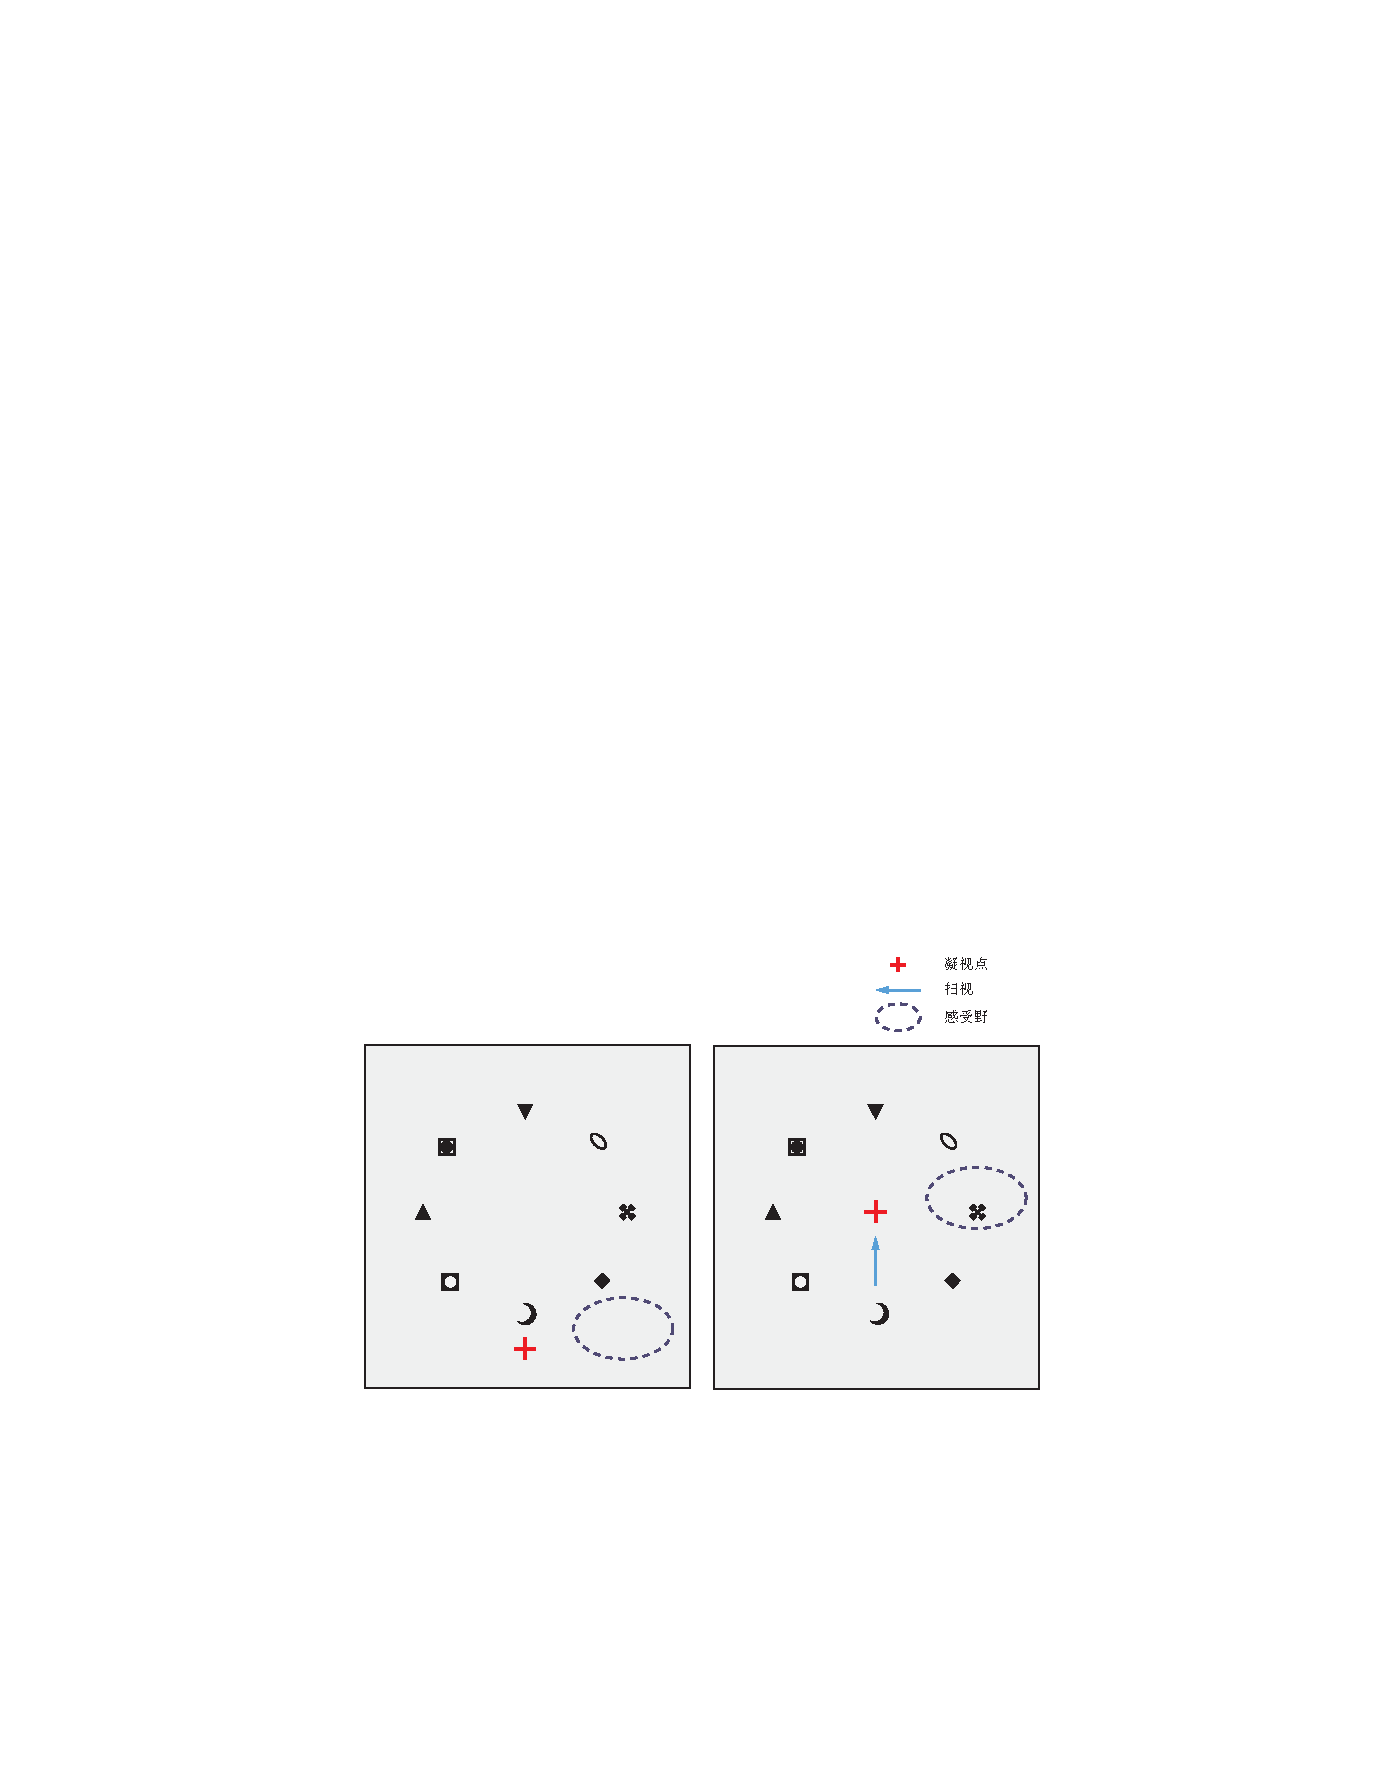
\includegraphics[width=0.83\linewidth]{chap25/fig_25_10}
	\caption{探索一组稳定的物体。
		猴子观看一个屏幕,屏幕上有许多物体在整个实验过程中都保持不变。
		猴子的凝视可以定位为使任何物体都不包括在神经元的感受野中(左),或者猴子可以进行扫视,将其中一个物体带入感受野(右)。}
	\label{fig:25_10}
\end{figure}


\begin{figure}[htbp]
	\centering
	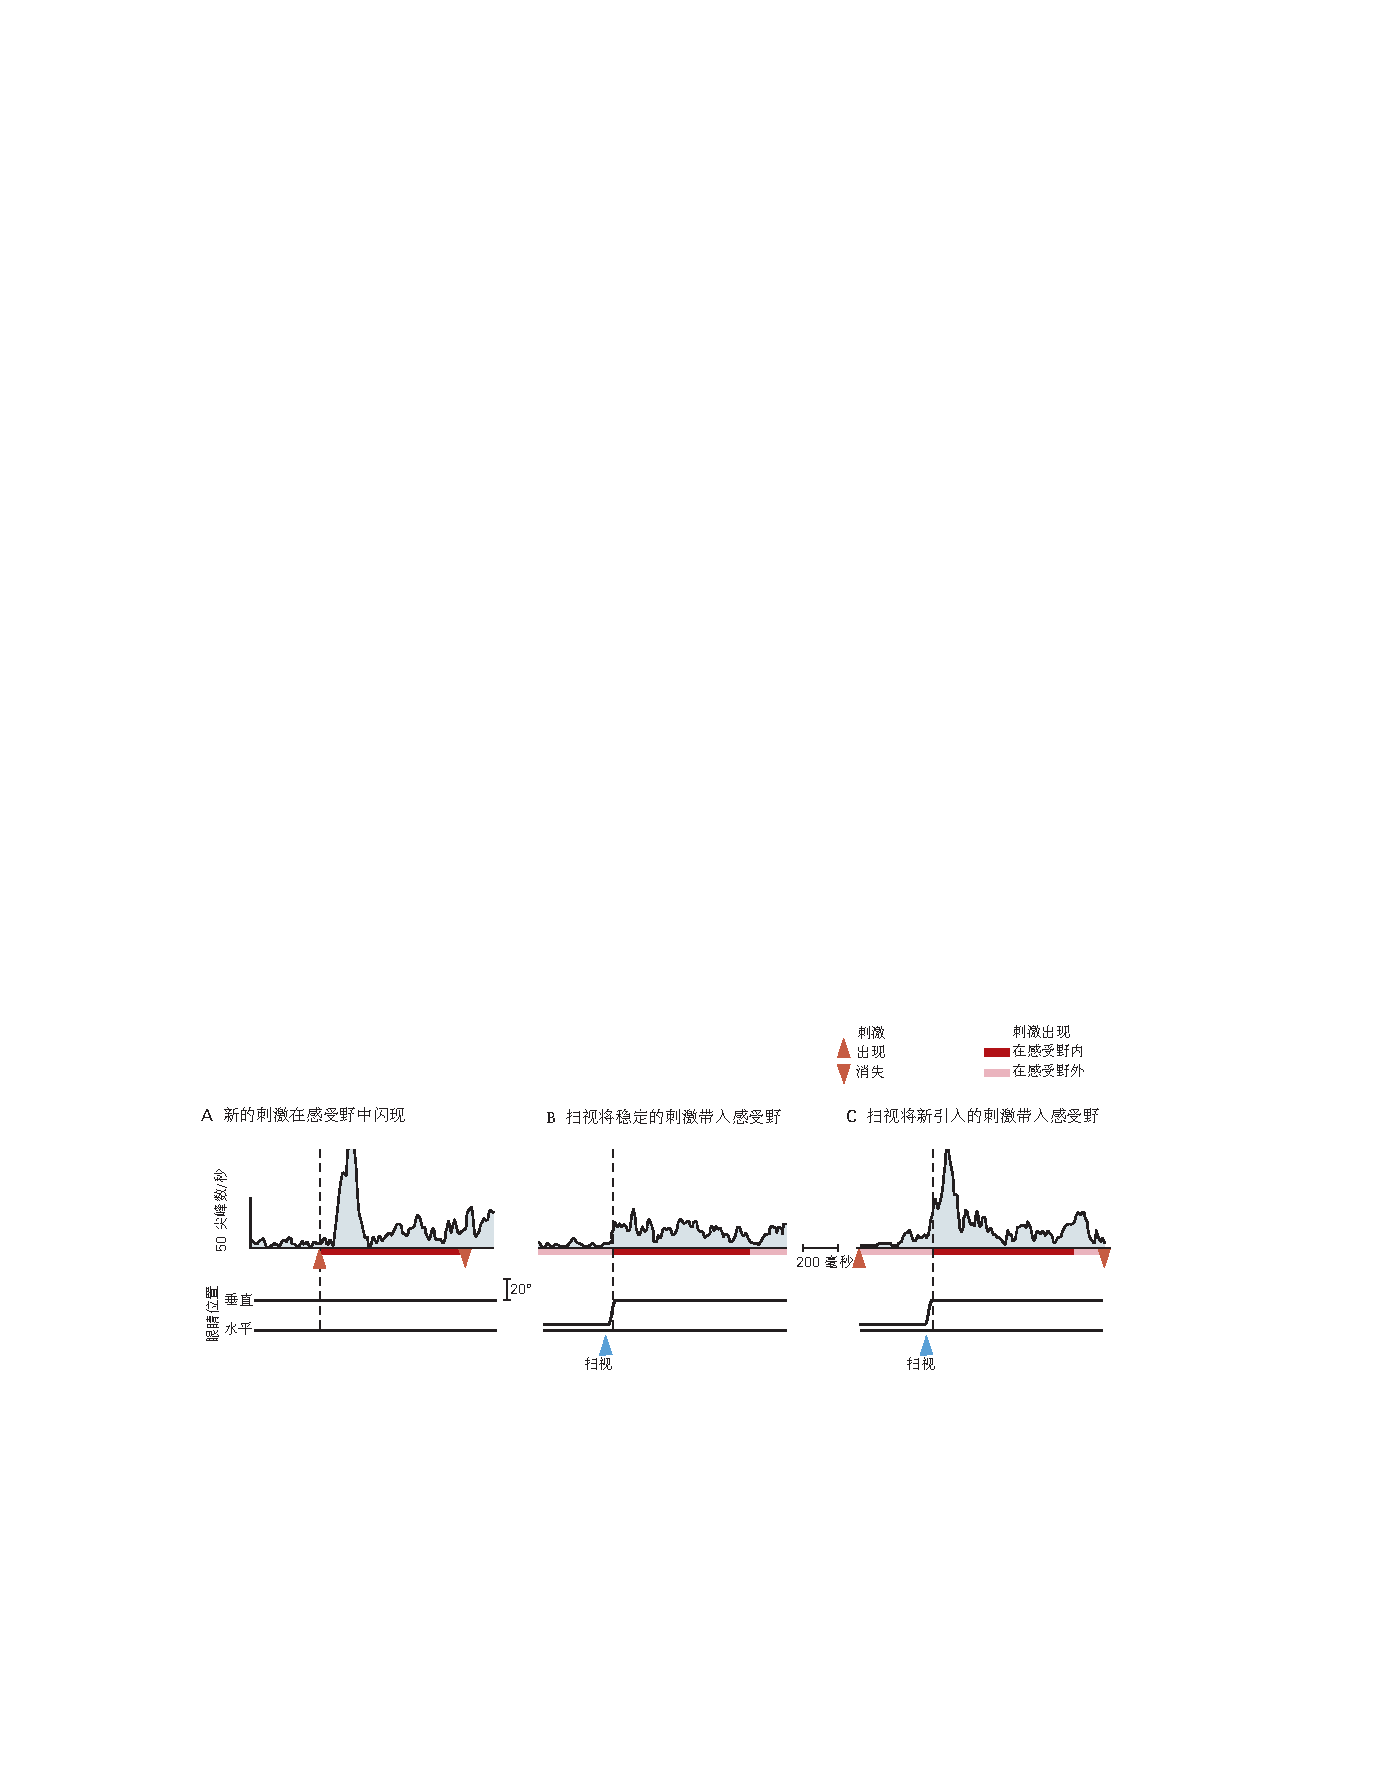
\includegraphics[width=1.0\linewidth]{chap25/fig_25_11}
	\caption{顶内外侧区域的神经元仅在对显著刺激做出反应时才会放电。
		在每个面板中,神经元活动和眼睛位置都是随时间绘制的。
		\textbf{A.} 猴子注视时,感受野中会闪现一个刺激。
		\textbf{B.} 猴子扫视,将稳定的、与任务无关的刺激带入感受野。
		\textbf{C.} 猴子做一个扫视动作,将最近闪光的位置带入感受野。}
	\label{fig:25_11}
\end{figure}


\begin{figure}[htbp]
	\centering
	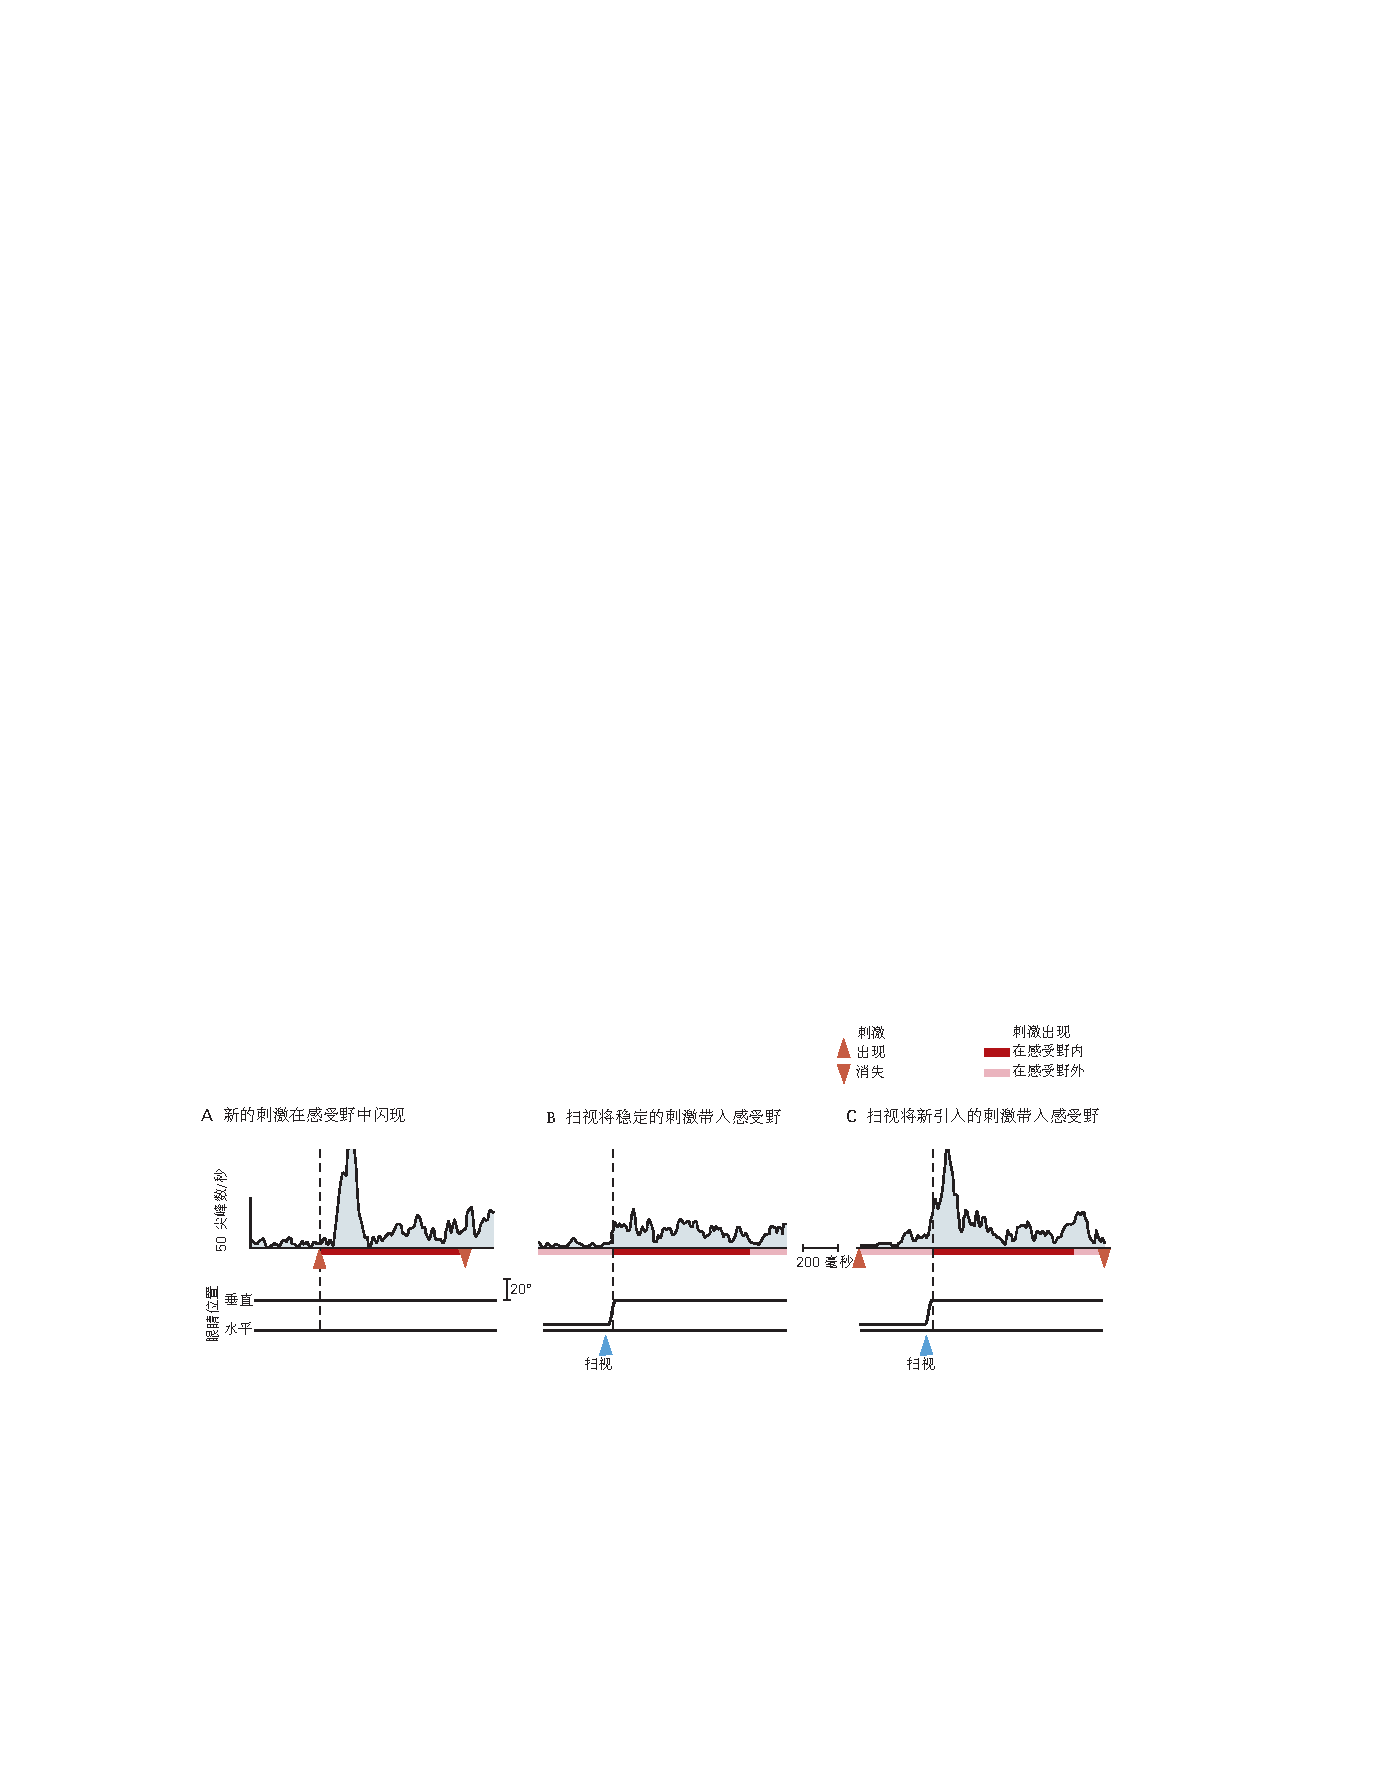
\includegraphics[width=1.0\linewidth]{chap25/fig_25_11}
	\caption{在扫视一个重要的稳定物体之前,位于顶内外侧区域的神经元会启动。
		在每次试验中,稳定阵列中的一个物体对猴子来说都很重要,因为猴子必须对它进行扫视。
		猴子固定阵列外的一个点,与阵列中的物体匹配的线索出现在神经元的感受野外。
		然后,猴子必须扫视阵列的中心,再扫视与线索匹配的物体。
		显示了两个实验(在A和B部分中)。
		左侧面板显示神经元对感受野外提示出现的反应,中间面板显示第一次扫视将提示目标带入感受野后的反应,右侧面板显示第二次扫视前对提示对象的反应。
		为了清晰起见,这里的提示是绿色的,但在实验中是黑色的。
		在两个实验中,扫视时的视觉场景是相同的。
		\textbf{A.} 训练猴子对提示的物体进行第二次扫视;
		当第一次扫视将物体带入感受野时,细胞会强烈地激发。
		\textbf{B.} 训练猴子对感受野外的物体进行第二次扫视;
		当扫视将与任务无关的刺激带入感受野时,细胞激发的能量要少得多。}
	\label{fig:25_12}
\end{figure}



\section{顶叶皮层为运动系统提供视觉信息}

视觉与\textit{辅助运动皮层}和\textit{前运动皮层}相互作用,为运动系统的动作做好准备。
例如,当你拿起一支铅笔时,你的手指与拇指的距离是铅笔的宽度;
当你拿起一杯饮料时,你的手指与拇指之间的距离与玻璃杯的宽度相同。
视觉系统有助于在您的手到达物体之前调整抓握宽度。
类似地,当您将一封信插入邮槽时,您的手会对齐以将信放入邮槽。
如果插槽倾斜,您的手也会倾斜以匹配。


% Patients with lesions of the
顶叶皮层受损的患者不能仅使用视觉信息来调整他们的握持宽度或手腕角度,即使他们可以口头描述物体的大小或槽的方向。
相反,具有完整顶叶和腹侧流缺陷的患者无法描述物体的大小或其方向,但可以像正常受试者一样调整他们的抓握宽度和方向他们的手。
顶叶皮层中的神经元是操纵或移动物体所需信息的重要来源。
视觉引导运动背后的神经操作涉及识别目标、指定它们的特性,并最终生成运动程序来完成运动。
顶叶皮层中的神经元提供手指独立运动所需的视觉信息。


% The representation of space in
顶叶皮层中空间的表征不像初级视觉皮层中的\textit{视网膜脑图}那样被组织成一个单一的图。
相反,它至少分为四个区域(\textit{侧顶叶}、\textit{内顶叶内区}、\textit{顶内沟腹侧区}、\textit{前顶叶}),以适合各个运动系统的方式分析视觉世界。
这四个区域将视觉信息投射到控制个体自主运动的前运动和额叶皮层区域(图~\ref{fig:25_13})。


\begin{figure}[htbp]
	\centering
	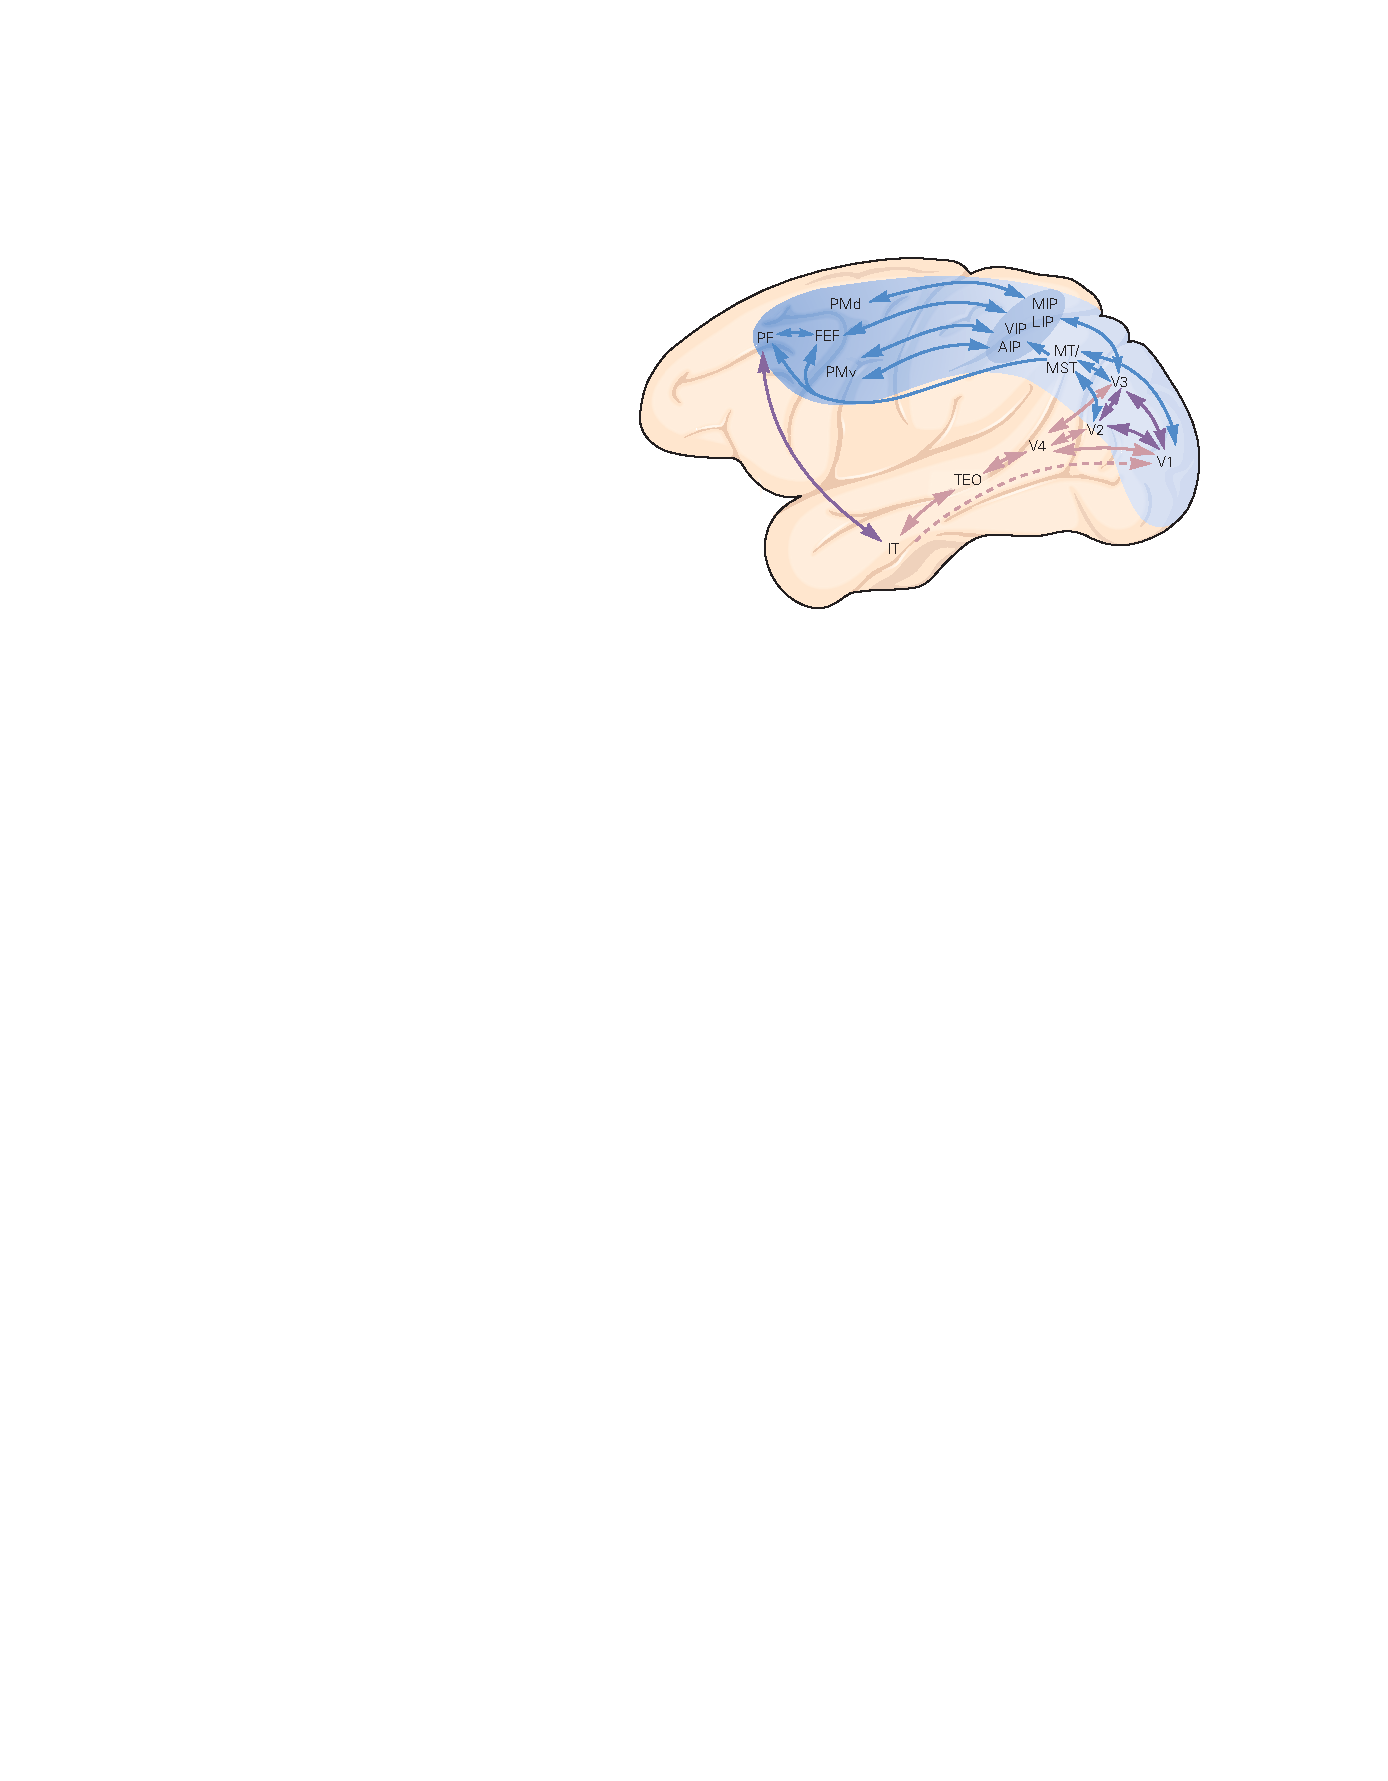
\includegraphics[width=0.7\linewidth]{chap25/fig_25_13}
	\caption{动作视觉处理的通路。
		背侧视觉通路(蓝色)延伸到后顶叶皮层,然后延伸到额叶皮层。
		腹侧视觉通路(粉红色)见第~\ref{chap:chap24}~章。
		从\textit{下颞皮层}到\textit{前额叶皮层}有双向投射。}
	\label{fig:25_13}
\end{figure}


\textit{内顶叶内区}的神经元描述伸手可及的运动目标,并投射到控制伸手动作的运动前区。
\textit{前顶叶}的神经元会发出可抓取物体的大小、深度和方向的信号。
该区域的神经元对可能会成为抓取运动目标的刺激做出反应,并且当动物进行运动时,这些神经元也会活跃(图~\ref{fig:25_14})。
\textit{侧顶叶}神经元指定\textit{扫视}的目标,并投射到\textit{额叶视区}。


\begin{figure}[htbp]
	\centering
	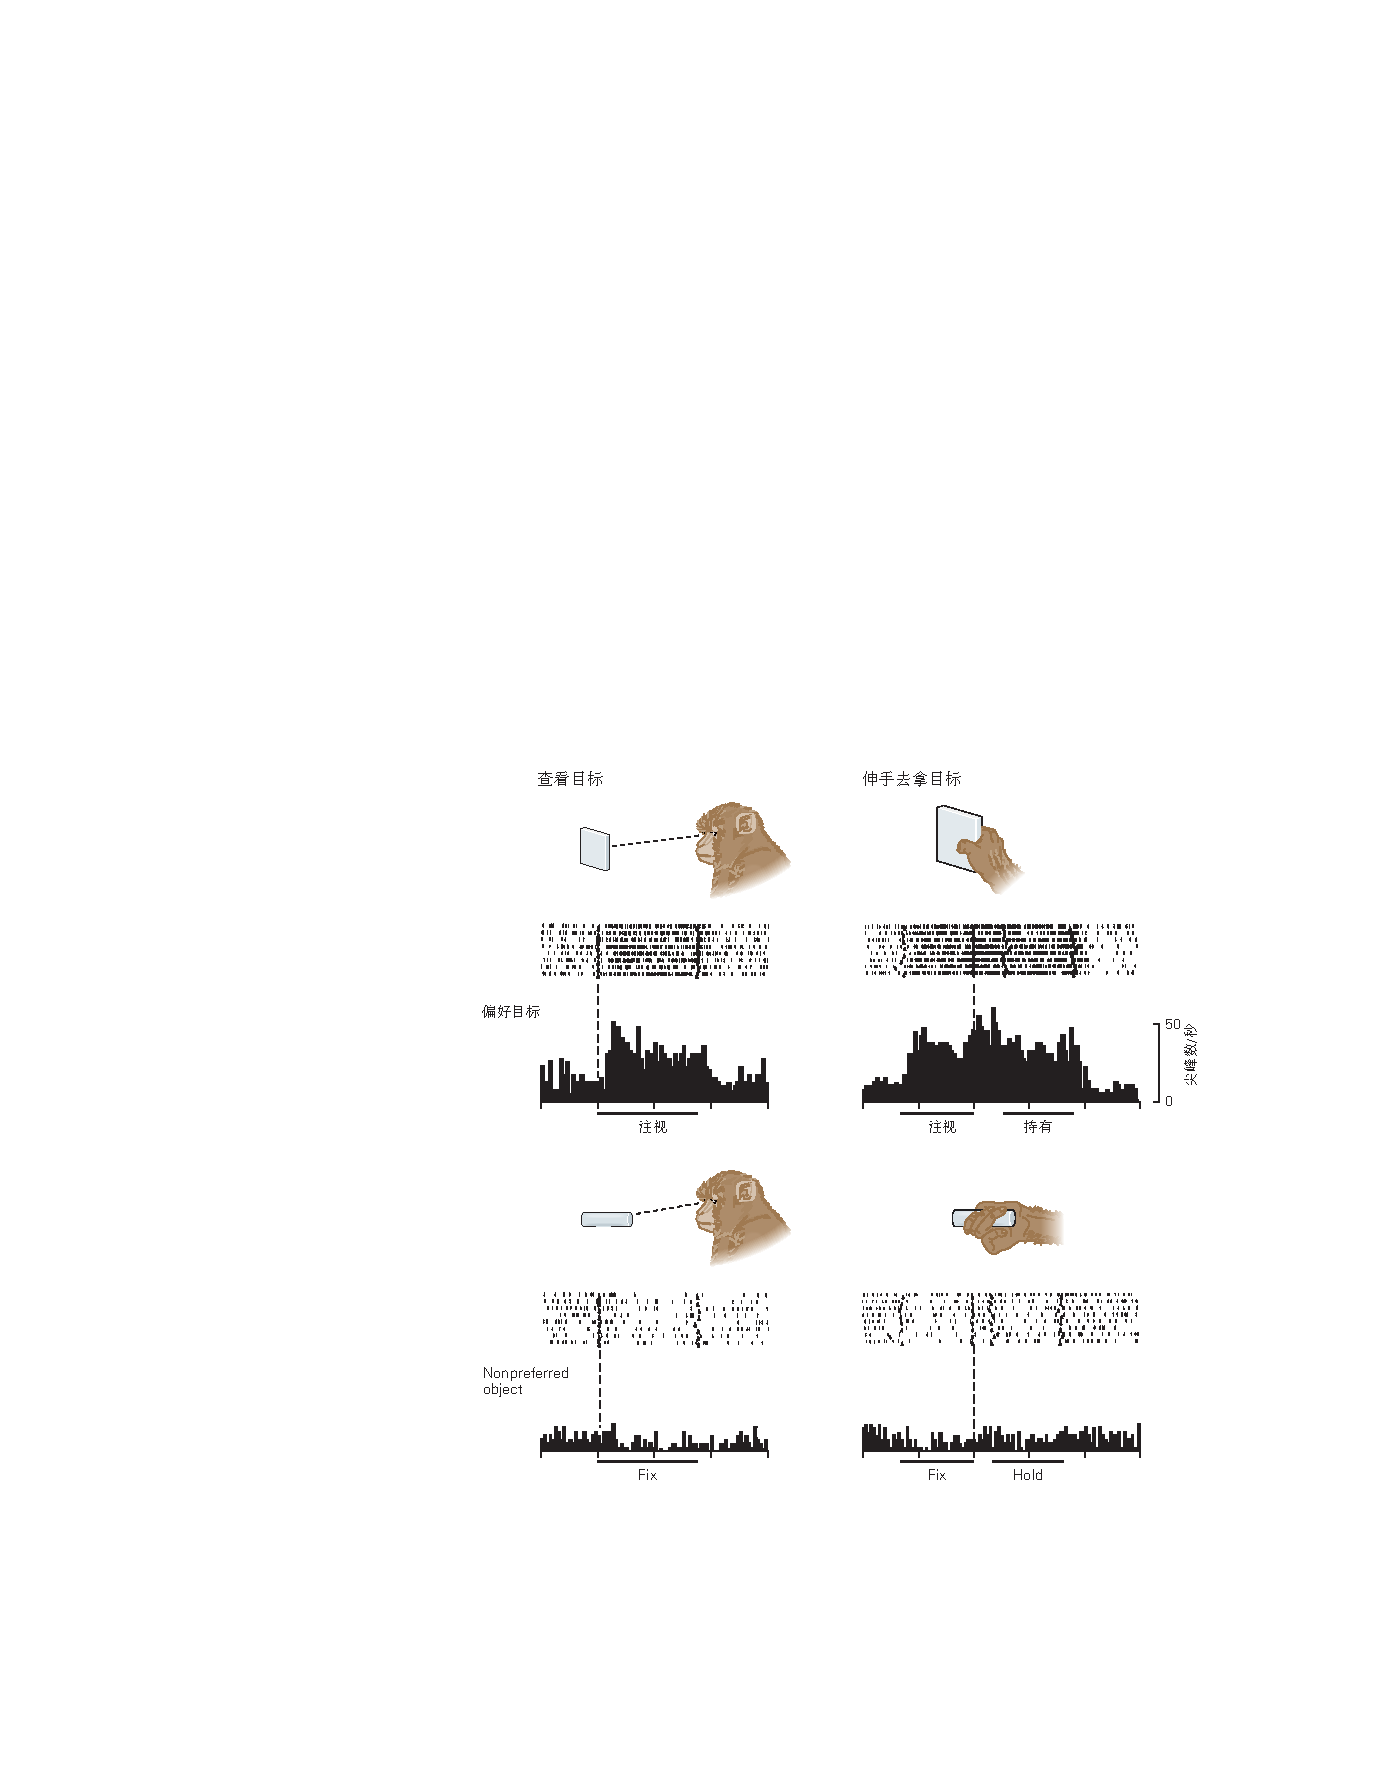
\includegraphics[width=0.87\linewidth]{chap25/fig_25_14}
	\caption{顶内前皮层的神经元对特定的形状有选择性的反应。
		这里显示的神经元对矩形是有选择性的,无论是观察物体还是伸手去够。
		无论哪种情况,神经元都对圆柱体没有反应。}
	\label{fig:25_14}
\end{figure}


因为猴子看不到它的嘴巴,\textit{顶内沟腹侧区}有\textit{双模态神经元},它们对面部的触觉刺激(图~\ref{fig:25_15})和视觉世界中接近触觉感受野的物体做出反应,使大脑能够估计靠近嘴巴的物体。
\textit{顶内沟腹侧区}投射到\textit{前运动皮层}的面部区域。


\begin{figure}[htbp]
	\centering
	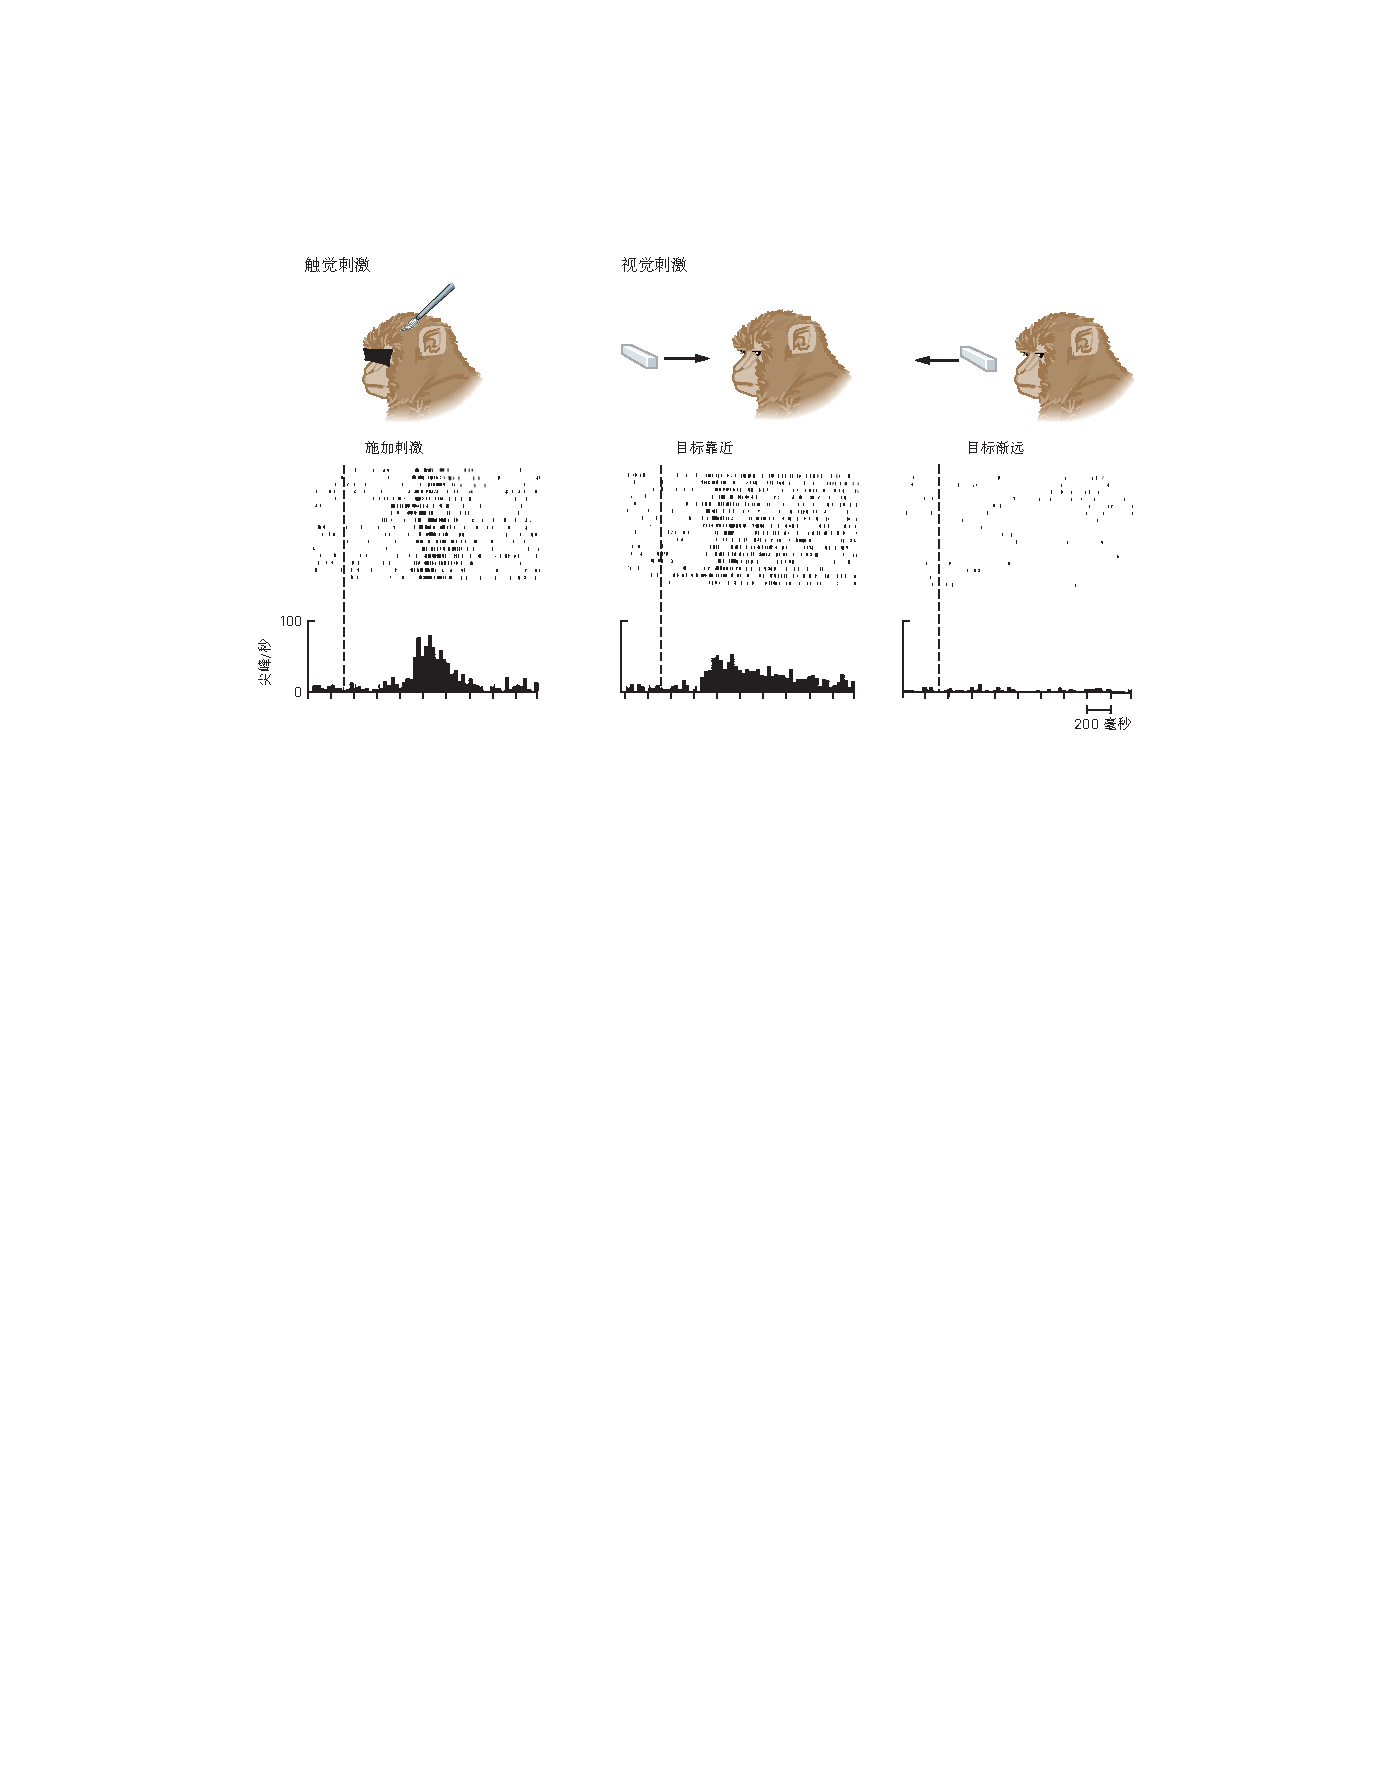
\includegraphics[width=1.0\linewidth]{chap25/fig_25_15}
	\caption{猴子顶内皮层腹侧的\textit{双模态神经元}对视觉和触觉刺激都有反应。
		这里显示的神经元对猴子头部的触觉刺激或朝向头部的视觉刺激做出反应,但对远离头部的相同刺激没有反应。}
	\label{fig:25_15}
\end{figure}



\section{要点}

1. 世界的图像通过眼睛进入大脑,眼睛在头部不断移动。
视觉系统必须补偿眼睛位置的变化,以根据视网膜位置计算空间位置。
\textit{亥姆霍兹}假设大脑通过将驱动眼睛的运动信号反馈到视觉系统来解决这个问题,以补偿眼球运动的影响。
这种对视觉系统的运动反馈称为\textit{伴随发送}。


2. 向动眼神经系统提供视觉信息的\textit{侧顶叶}神经元显示了这种\textit{伴随发送}的证据。
如果即将发生的\textit{扫视}将刺激带入其感受野,通常不会对空间中的特定刺激做出反应的神经元将对其做出反应。


3. 这种感受野重新映射取决于从上丘中间层到丘脑内侧背核再到\textit{额叶视区}的通路。
内侧背核失活会损害猴子在扫视后识别眼睛落在何处的能力,这表明\textit{伴随发送}具有感知和运动作用。


4. \textit{谢林顿}假设大脑使用眼睛位置根据物体图像在视网膜上的位置来计算物体的空间位置。
体感皮层中有眼睛位置的表示。
眼睛位置调节顶叶神经元的视觉反应,空间中的目标位置很容易从这种调节中计算出来。


5. 一个悬而未决的问题是大脑如何在眼睛位置和\textit{伴随发送}机制之间进行选择以确定空间位置。
因为\textit{伴随发送}先于眼睛位置的变化,本体感觉紧随其后,所以大脑可以在不同时间使用这两种位置吗?


6. 注意力是大脑选择世界中的目标进行进一步分析的能力。
没有注意力,空间感知就会受到严重限制。
例如,人类很难注意到视觉世界的变化,除非他们的注意力被吸引到变化的空间位置。


7. 顶叶皮层神经元的活动预测了猴子的空间注意力,这是通过它们的感知阈值来衡量的。
顶叶皮层将许多不同的信号(运动信号、视觉信号、认知信号)相加,以创建视野的\textit{优先级图}。
运动系统使用这张图来选择运动目标。
视觉系统使用相同的图来寻找视觉注意力的轨迹。


8. 顶叶皮层的损伤导致对侧视觉世界的忽视。


9. 顶叶皮层提供的视觉信息使运动系统能够在手实际落在目标上之前调整手的握力,以匹配其到达的物体的大小。
相比之下,由于下颞皮层损伤导致知觉缺陷的患者可以很好地调整他们的抓握,即使他们无法完美地描述他们所触及物体的种类或大小。


10. \textit{顶内沟}中至少有四种不同的视觉地图,每一种都对应于特定的运动工作区。


11. \textit{前顶叶}的神经元对\textit{抓取}目标作出反应,即使猴子在完全黑暗中进行抓取动作时也会作出反应,并投射到\textit{前运动皮层}的抓取区域。


12. \textit{顶内沟腹侧区}的神经元对靠近\textit{嘴巴}的物体做出反应,在面部有触觉感受野,并投射到\textit{前运动皮层}的嘴巴区域。 


13. \textit{内顶叶内区}的神经元具有\textit{手臂位置的表征}并对\textit{到达的目标}做出反应。


14. \textit{侧顶叶}的神经元对眼球运动目标和视觉注意目标作出反应,在眼球运动前放电,并具有\textit{眼球位置的表征}。
这些神经元的活动受眼睛在眼眶中位置的调节。


15. 体感皮层 3a 区面部区域的神经元具有眼球在由对侧眼产生的眼眶位置的表征。

